\documentclass[10pt]{scrartcl} 

\renewcommand{\baselinestretch}{1.15} 

\usepackage[english]{babel}
\usepackage[utf8]{inputenc}  

\usepackage{import}
\usepackage[smaller]{acronym}
\usepackage[export]{adjustbox}
\usepackage{amsmath}
\usepackage{graphicx}
\usepackage{natbib}

\usepackage{pdfpages}
\usepackage{float} 

\usepackage{listings}
\usepackage{color}

\lstset{frame=trlb,
  language=Python,
  aboveskip=3mm,
  belowskip=3mm,
  lineskip={-3.5pt},
  showstringspaces=false,
  columns=flexible,
  basicstyle={\small\ttfamily},
  numbers=left,
  numberstyle=\tiny\color{gray},
  keywordstyle=\color{blue},
  commentstyle=\color{dkgreen},
  stringstyle=\color{mauve},
  breaklines=true,
  breakatwhitespace=true,
  tabsize=2
}

\usepackage{geometry}
\geometry{a4paper,left=30mm,right=30mm,top=25mm,bottom=35mm}                    

 
\begin{document} 

\title{RayTrashing Report}
\author{\small Alexios Stavros Stellas, Srinath Panchavati Ramakrishna, Nikolaos Kyknas, \\ \small Sebastian Klaus Köhler, Stamatios Stampelos,Farhad Saghab Gandomabadi}
\date{28 March 2018}

\maketitle

\section{Introduction}
Every human has multiple senses that he uses on a daily basis. One of the most important is vision. Everything that is located in a person’s field of view is basically an interaction between him and that object. Since the person is not touching anything in his view, some would argue that there is no actual interaction. However, when an electromagnetic wave leaves the light source and hits an object it reflects from it. Our eyes catch these reflected waves which carry information and our brain uses them in order to create an image. This proves that there is an interaction between the object and the observer. \par
This is a very amusing and simplistic way of explaining how ray tracing works. Yet, there are some notable differences. Rays are sent from the observer’s point of view (camera or eye) towards a specific pixel in the image. If the ray meets an object then a secondary ray is reflected towards the light source with the intention of finding out how much light this specific pixel receives. If another object is hit on the way to the light source this simply means that this part of the object in in shadow. Even though this is only a basic version of what the team actually tried to recreate and achieve, it gives an overview of the whole process. Each member of the group contributed in creating a ray tracer that included these processes mentioned above but also much more.\par
 The ray tracer was improved in order to include multiple objects in the scene including spheres, cubes, cylinders,cones and planes. Additionally on top of the shadows that are cast from objects obstructing the light source, more interactions have been added on how the objects react to the light with the aim of making everything more realistic. These additions include the reflectivity of the object and how much light bounces off from its surface which subsequently includes specular reflection and diffuse reflection based on the surface of the object.  Translucency was similarly achieved allowing us to create objects that have various degrees of transparency each one allowing more or less light to pass through them. All these additions permitted for a more realistic and suitable ray tracer to be developed.  The entirety of these processes happen in the backend. \par
However, all of them would be useless without an interface that would allow the user to interact with the ray tracer. The front end team has accomplished to create a graphical user interface (GUI) that is user friendly and which interacts fully with all the backend processes. This provides a ray tracer with improved usability, allowing the user to use the program without having to understand every little detail of the coding process. The GUI includes a visual representation of every object in the scene with a simple but elegant canvas, providing the user with a guideline of how the scene which he attempts to create looks like. This visual allows the user to have a better understanding of what he attempts to create. Multiple values are provided in the GUI for the user including everything that was mentioned before like reflection, translucency but also a selection of every colour that the user can choose to embody in each object. The fast responsiveness and user friendly environment of the Front end with the combination of the realism and practicality of the backend allowed for the creation of an extraordinary application.\par


\section{Review}
Ray tracing in computer science has existed for quite some time. This means that multiple attempts to create a ray tracer exist online either by big companies focusing on graphics or even individual people. Depending on the budget and time that was available many different ray tracers are created ranging from a minimal level of tracers that can maybe only render a sphere to tracers that produce a rendered outcome that is very difficult to distinguish from real pictures. \par
One that is worth mentioning is POV-Ray, which has a high popularity.  The first ever version of the software was released back in 1991 making it one of the oldest products in the market related to ray tracing. Its popularity was that high that in 2002 POV-Ray became the first tracer that rendered an image while in orbit inside the international space station. \par
Over the years multiple features were added to POV-Ray increasing its capabilities exponentially when compared to the initial release.  The product has even included in a recent update environmental effects like smoke or clouds. This is something that wasn’t even feasible 27 years back for such kind of software. All these additions accumulated over the years, each one making the rendered image more realistic each time. Finally by the use of multiprocessing and increased power that came with improved hardware the device became much faster in the recent years.\par
In the following years other companies decided to move down the path of ray tracing. One that everyone has heard is NVIDIA, even in cases of people who have no idea what ray tracing is. Mental Ray did not originally belong to NVIDIA but it was part of the company Mental Images which is now owned by NVIDIA. The realism that this software can create has been so incredible that it has been used in many major Hollywood movies.\par
Finally, in terms of commercial software that supports ray tracing TracePro cannot go unmentioned. It is so useful that even NASA uses it for many purposes, especially since it is very useful for many aerospace projects. NASA even provides LAMBDA Research Corp. with a grant allowing them to grow and improve it even more. LAMBDA Corp. has been continuously developing TracePro from 1994.\par
All this kind of popular applications can be used for many different reasons in the graphics community, each one providing a better experience for the user along with a platform that can create basically anything, only limited by the imagination of the user and time. However, these applications are not only limited to ray tracing. It is easy to see that multiple individuals have tried to create numerous ray tracing applications on the internet from scratch or by improving already existing models.\par
Plentiful tutorials exist allowing basically anyone with time and a basic knowledge of coding to construct a simple ray tracer. An easy search provides anyone with hundreds of different attempts to create a ray tracer. C++ appears to be the preferred chosen method for developing a ray tracer in most cases. Some even claim that a very simple ray tracer can even be created in less than half an hour.
In comparison our own ray tracer might not be as capable and realistic as the commercial software that was discussed. Let’s not overlook the huge budget, time and workforce that those companies had to their disposal.  \par

\section{Requirements \& Design}
Our first steps in regards with the ray tracer, included building a plan of what the final result would look like and the features it will include. After the team made a plan and a timetable that it had to stick with, we started programming the tracer. For the beginning the plan included the creation of a ray tracer that had all the minimum requirements that were essential to the project, followed by the speedy implementation of extra features based on the result that was wanted and the remaining time. \par
This included the creation of basic shapes like the sphere and cubes which could be given 3 dimensional coordinates, change colour based on the users preference and had translucency as an option, so the user could make them as transparent as needed. After the time that the team would manage to meet all the minimum requirements work would focus on the addition of various features which were thought at the beginning of the project, that would add extra realism and finesse to the ray tracer. \par
One of the very first additions which were given priority was the creation of shadows that any of the objects might cast depending on the position of the light in the scene. Since light affected this step so immensely the ability to add multiple light sources was also added to the plan. Reflection was also a major advancement in the quality of the project so it had to be included. This meant that the objects had to be given the ability to reflect a specific amount of light, depended on the user, but at the same time the reflected light had to interact with the rest of the objects. Further shapes also had to be included. On top of the sphere and cube, a cylinder but at the same time a plane were highly desired. \par
Apart from all this additions the ray tracer also had to be fast and functional. Creating a tracer that is extremely slow or doesn’t respond properly would inflict a great deal of damage to the usability of the application even if it included every single feature that it’s humanly possible. This meant that the code had to be optimised. Even if that would contribute greatly, this would not be enough to achieve the desire effect. The team’s vision was to give the tracer the ability to render shapes within 30 or 40 seconds. The only way that we could achieve this increase of the speed with the tracer, was by using multi-processing, which would cause the rendering process to expedite considerably.\par
All that of course only briefly explained about the plan that was created in regards to the backend. However, a strategy was also needed for the creation of the frontend. Both the backend and the front end had to be compatible by using the same values. This would majorly increase the chances of merging the two parts into one single application without having any conflicts but at the same time avoid mistakes in the user input, for example by misplacing objects and so on.\par
Now in terms of the frontend we needed a design that was elegant but at the same time simple to use by anyone. The page had to include an interface that would receive all the expected values needed for the backend from the user. At the same time it would provide a simple example of how the scene would look like after rendering. This way the user had a pretty good idea about where the objects will be located in the scene and how they will be placed relative to the user’s viewpoint. Creating an environment that was faultless for the user was essential since it is the first interaction that an operator has with our ray tracer.\par
Drag and drop was a group preference that was thought right from the beginning. We wanted the user’s experience to be as simplistic as possible, basically making the tracer usable by even a child. The user could simply drag and drop objects into the scene, placing them wherever it’s convenient without needing to have any specific knowledge on the exact coordinates. This would also allow for a more perfectly constructed scene, reflecting the user’s exact plan.
The goal of the project was to create a scene that could be as realistic as possible with only minimum effort from the user’s part. Following and completing aims that were set from the start provided a gradual and steady progress with the tracer’s capabilities increasing more and more each week. In the end the final product was fairly realistic and adaptable . There are additions that can still be implemented in the future to make the result even better, but for the specific timeline we feel satisfied with the result we ended up with.\par

\section{Architecture}

One of the requirements of the Ray Tracer was to have two separated applications. A frontend application, where the user can create a scene and a backend where the user can upload and render the created scene. To fulfill the requirements we decided to develop a client-server architecture. For the communication between the client and the server we used the Hypertext Transfer Protocol (HTTP). Because of the high-level abstraction we profit from the reliability and statelessness compared to a low-level socket implementation. Furthermore, using this architecture would easily allow us to use multiple backend servers and load balancing. Wrapping the communication in HTTP also improves the security. Instead of using plain HTTP we could use HTTPS to encrypt the communication. Figure \ref{fig:architecture} gives an overview of the architecture. 

 \begin{figure}[h]
  \centering
  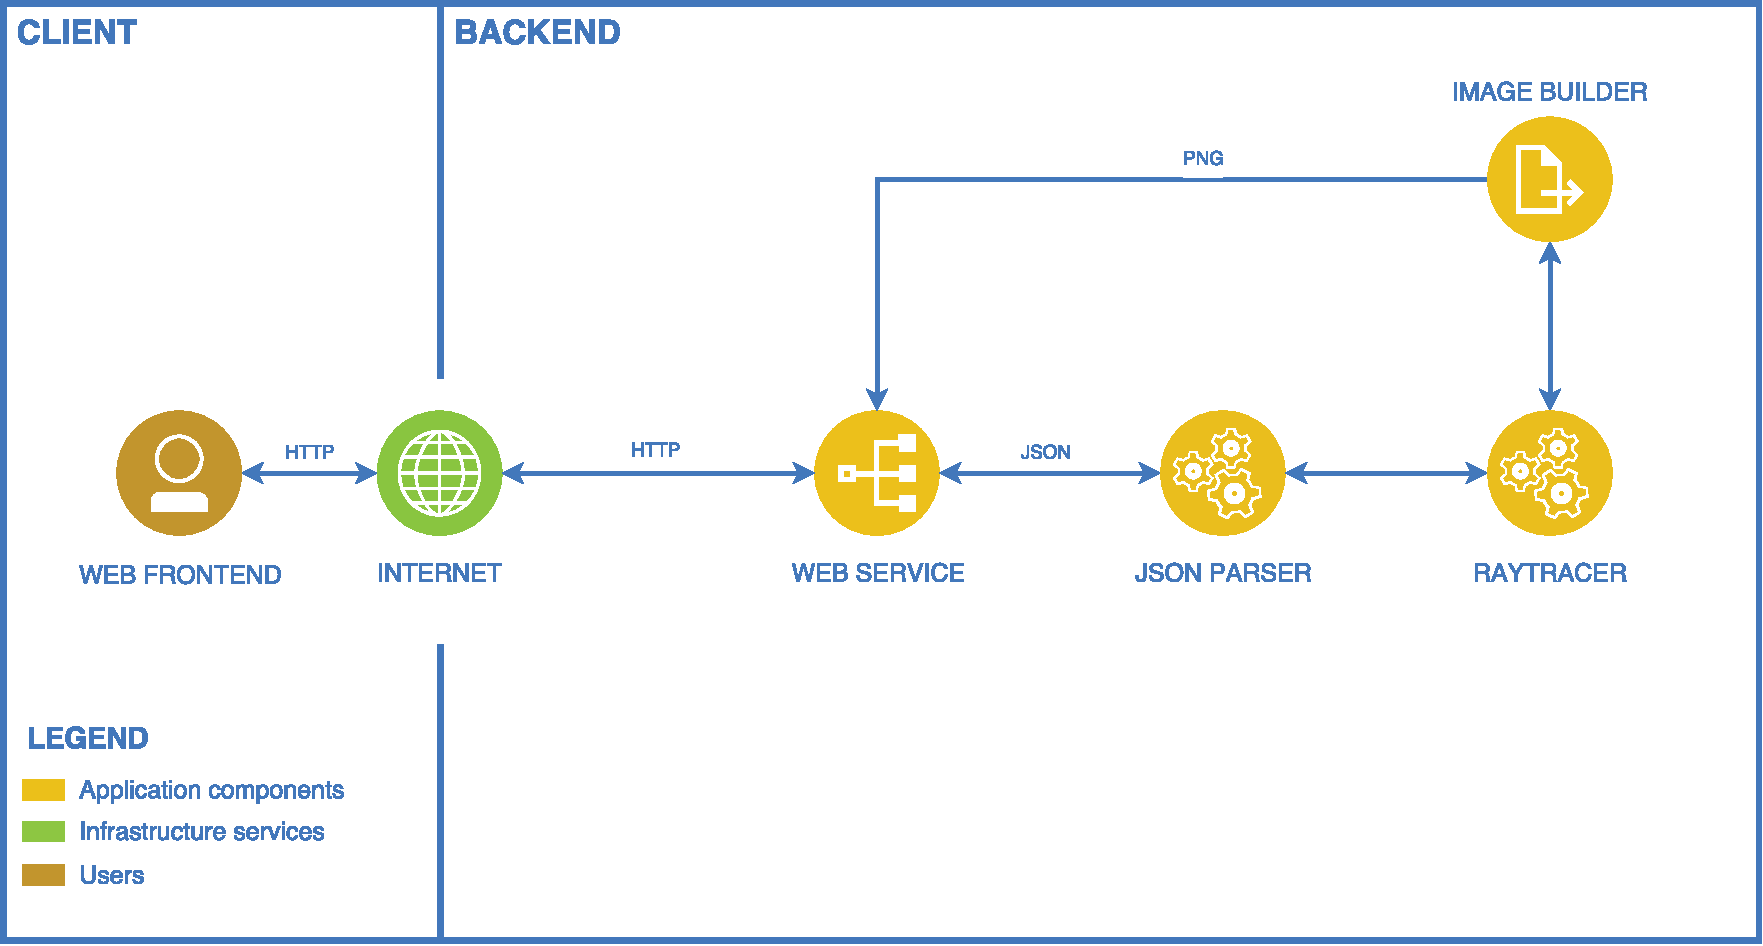
\includegraphics[width=0.85\textwidth]{images/architecture.pdf}
  \caption{Overview of the Architecture} 
  \label{fig:architecture} 
\end{figure}

Another advantage is the expandability. Instead of using a browser as a frontend we could develop a mobile application to communicate with the backend.

\subsection{Frontend}

Frontend for this project serves the purpose of enabling the user create a 2D scene which is the representation objects and their relative coordinates. User is also able to configure the information about the lights that are present in the scene. After the preferred scene is constructed, pressing the Render button will send the data from the front-end to the back end using JSON. The JSON data is later used by the back-end for creation of a 3D model in accordance with the created scene on the front-end. After creation of the 3D model in back-end the response will be sent to front-end in the form of a binary file which will be used to construct the image and show it to the user in the provided window. \par

Creation of the 2D scene in the front end and passing the information from the front-end to back-end has been achieved using the following web technologies:
\begin{itemize}
    \item JavaScript
    \item jQuery
    \item HTML 5
    \item CSS 3
    \item JSON
\end{itemize}

The role of each technology in this project will be explained in detail in the following sections after explaining the main features and functionality of the project.

\subsection{Features and Functionality}
Adding shapes, lights and other settings can be done using the navigation buttons on the left hand side of the front-end. These navigation buttons pull out boxes which contain the required input boxes and lists. Each button invokes a different box like the first navigation button with light bulb on it invokes the box which has implementation related to lights and the shapes button invokes the box which has the functionality required for adding shapes. There is also a third button which is for general settings like adding a floor, camera etc. When a button, which has invoked a box, is clicked on again, it collapses the box and goes back to the initial position. There can only be one open box at a time.
\subsubsection{Adding Shapes}
After clicking on the shapes navigation button, the user can add multiple shapes including Sphere, Cube, Cone, Cylinder and Plane to the scene both by clicking on the shape icon or by typing the coordinates and size. The colour of the shape can be selected using the colour picker. After the required shapes are added, pressing the \textit{Add Shape} button will add the shapes to the scene. After adding the shapes user is able to see the added shapes on the scene and can use the right hand side shape list of the added shapes. User is able to change the coordinates and size of the shapes after they are added to the scene and also delete the shapes if required. If the user wants to clear the grid, it can be done using the \textit{Clear Grid} button. In the front-view of the scene, the user gets the additional functionality of being able to drag the shapes wherever he/she wishes to inside the canvas.\par
There are other features as well:
\begin{itemize}
    \item Reflection and Specular Reflection \par
User can use the range selectors on the front-end to determine the reflection and specular reflection of the objects on the scene.
    \item Material \par
    User can choose the material of the shape from the drop-down list. Each selection will change the values of Reflection, Specular and Transparency to some preset values. This is done to help the user understand what values each range has to be set to so that the intent of the material selected is realized.
    \item Refractive Index \par
User can specify the refractive index of the shapes. This shows how the rays pass from different media like air, water, glass, etc. and how they get refracted.
\item Transparency \par
User can use the range selectors on the front-end to determine the transparency of the shapes.
\end{itemize} 

\subsubsection{Add Lights}
User can add multiple lights to the scene by typing the preferred coordinates and pressing \textit{Add Light}, after clicking on the lights navigation button. User can also see the list of all lights added to the scene on the light list provided on the right hand side of the screen. He/She can also use the range selectors to select the brightness and ambient light of the scene.

\subsubsection{Other Settings}
If the user wants extra functionality, then he/she can click on the settings navigation button to pull a box which has the following features: \par
\begin{itemize}
    \item Add Floor: A floor or a plane to the scene can be added by just checking a box.
    \item Add Room: A room can be added to the scene by checking a box. User can, at a time, only choose either a room or a floor. Adding room adds floor as well by default. The user has the ability to choose neither as well if he/she wishes.
    \item Specify Image Size: If the user wants to generate a bigger image, then he/she can select the image size on the drop-down list and render the image. The largest image size which can be rendered is 1000*1000 pixels (width * height) and the smallest is 500*500.
    \item Configure Camera: The user has the complete liberty of selecting how to view the rendered image. He/She can select one of the provided options, viz., front view, top view and right side view. If the user wants to, he/she can click on the \textit{Advanced Camera} button to specify the preferred positioning of the camera, direction and right angle values.
    \item Anti-Aliasing: Anti-Aliasing is used to smoothen the rendered image up and the user has the capability of choosing whether to do it or not .
    \item Specify File name: The user can specify the preferred file name for saving the image after the rendering has finished. When the user downloads it, the file will be saved in the Downloads folder with the name specified in this field. 
\end{itemize}

\subsubsection{Views}
There are 3 views in the front-end of the project. Front, Top and Side view. Front view is the view that represents what the scene looks like when looked at from the front and is the view that allows dragging of the shapes. Side view shows what the scene would look like if you were to look at it from the right hand side. Top view is the view that works as of you are looking at the scene in the front view while you are sitting, but you decide to stand up and loot at the shapes from the top. From front view to top view the Z value of the object becomes Y value by calculating how much movement has happened in the Z axis. This is translated to relative values we use for the canvas (coordinate ranges are from 1 to 3). As for the size of the object, if we moved in Y axis we calculate the shape size based on how much we moved and multiply that by a constant (60.38) to make the shape match the functionality at the back-end. The constant has been found by trial and error. From the front view to side view we perform the exact same calculations with the exception that Z value is X coordinate of the shape and X value is size of the shape. 

\subsubsection{Changing and Deleting Shapes and Lights}
List of all the shapes and lights added to the scene can be views on the right hand side of the front-end. When a shape or light is selected from the select box we are accessing all the information related to the shape or light object and we populate the relevant text boxes so we can later change the values of the particular object. The advantage of this functionality is that we will see the shapes and lights getting added in real-time. In the case of the shapes, the colour of the specific shape is also highlighted with the name of the shape. This helps in identifying the exact shape for any further modifications. If the user unintentionally added a shape outside the canvas, he/she can just click on the shape and bring it back into the canvas by just changing the coordinates in real-time. Also if we decide to delete and individual shape, we can delete it from the scene by just selecting the shape and clicking on \textit{Delete} button. \par

Changing size of the shapes is also possible. The user can change the size of the object by selecting the shape and changing the size value in the size text box and pressing the \textit{Change} button. \par
In case user prefers to clear the grid without refreshing the page, pressing the \textit{Clear Grid} button will remove everything from the views and object representation lists on the right hand side. The JSON is also cleared and rendering at this point will retrieve a blank image from the back-end. 

\subsubsection{Dragging the Shapes}
There are two ways for changing the coordinates of the shapes: 
\begin{itemize}
    \item By using the provided text boxes, changing their value and pressing the \textit{Change} button. When we press the \textit{Change} button and the values associated with the selected object will be replaced and all the objects will be redrawn again. This the same case with the lights as well as their coordinates can be changed by following the same procedure.
    \item By dragging the created object which only works in the front view. Dragging is performed in several stages, stage one is the mouse-down which captures the location of the mouse and we check if the click has been made on the canvas. We then convert the raw values from the screen to relevant values that we can use to create shapes and by relevant, we mean the center of the canvas. For us, center is at coordinates (0,0). At this point we have to check which shape it is that we are clicking on and we do that by going through every shape and check if we have a shape that matches the coordinates of the mouse click on the canvas. We do this by calculating where the edges of the shape would be by taking into consideration the center of the shape and its size and we use the same method for every other shape. Now we know what we are selecting and we go to the second stage which is the dragging. In this stage we place the original shape way outside the canvas and we show a temporary shape around the mouse pointer and when we perform mouse-up, we delete the shape that is outside the canvas and repaint the new shape around the mouse pointer. In addition, when we drag a shape outside the canvas we call the mouse-up function again and draw the shape on the edge of the canvas.
\end{itemize} 

\subsubsection{Responsive design}
Front-end of the project has been designed in a way that information in the views like shapes and lights will flow and re-size according to the size of the browser window of the user. The canvas has also been designed in such a way that it becomes smaller if the user re-sizes the window. The shapes inside the canvas also become smaller or larger according the size of the window set by the user. The navigation buttons on the left hand side also retain their responsive functionality when any sort of re-sizing happens.
\subsection{HTML 5}
HTML, Also known as hypertext markup language is the skeleton of our front-end design. We use HTML to put the major parts of the application related to creating the scene in place. Drop-Down menu, range selector,text boxes, check boxes, buttons, color picker and last but not least canvas tag are the major HTML elements used in the construction of front view of the project.

\subsection{CSS 3}
CSS also know as Cascading StyleSheet is used for arranging the different sections on the front end of the project. It is also used to create a more appealing look for the front-and of the project. The buttons, the background, the navigation buttons on the left hand side, etc. all have been styled using CSS3.

\subsection{JavaScript and jQuery}
JavaScript is the scripting language used by the front-end to perform several tasks such as retrieving the values from the HTML elements, drawing the shapes on the HTML canvas for the scenes, making the colour picker work, etc. All the calculations of the canvas, the coordinates of the shapes and the lights are all done in Javascript. jQuery is also used in the front-end to help with the functions and boil down the code to reduce the number of lines. \par
We have used the object-oriented feature of JavaScript to make every shape or light into an object. This gives the flexibility of adding any kind of feature to individual shapes. For example, in the case of Sphere, the parameter \textit{height} is not required but something like a Cylinder or Cone need \textit{height}. Hence, each of these shapes are objects of a parent class called \textit{Shape}. This also helped us add all the functionalities mentioned above with as little code changes as possible. We are reusing the code with the help of object-oriented approach and this saved us a lot of lines of code. We also have different \textit{js} files for different functionality. This helps in understanding the code better and gives the additional benefit of being able to search the required code efficiently.

\subsection{Integrating Back-End with Front-End}
JSON or Javascript Object Notation is the the data interchange format used in the front-end to collect the information related to the scenes and pass them to the back-end. After collecting the data from the scene and placing it in a JavaScript objects, a JSON object is created from these objects and passed to the back-end using XMLHttpRequest. By using the XMLHtpRequest we eliminate the need for saving the image on the server. At the end of it all, we receive the data (PNG image) from the back-end, which gets shown on the front-end. The adding of the JSON became very simple because of the use of classes and objects. Since each shape, light, and other major features are classes and objects themselves, converting and adding to the JSON is made easy. 

\subsection{Used Libraries}

We kept the usage of libraries to a minimum since we believed in programming everything from the scratch. jQuery and Farbtastic are the only libraries used for the front end of the project. jQuery functions are used in our JavaScript code to help with the tasks which would've, otherwise, been tremendously difficult to implement in plain JavaScript. Farbtastic is a color picker library to help the user easily select the color of shapes. This is a very intuitive and user-friendly feature in our product.

\section{Backend}

For the backend implementation we decided to use Python as a programming language because we wanted to use the chance to learn a new programming language during a real life project. Therefore we also tried to avoid third-party libraries and instead implement the whole functionality on our own. Of course we weren't able to completely avoid libraries and we had to use for example Django for the web service, numpy for the array calculations and math for basic calculations like square root.

\paragraph{Django}

To provide the necessary interfaces we decided to use the Django library for the web service. One advantage of Django are the countless default features it provides. Probably a smaller library would provide similar features, but we wanted to learn how to use Django and if we look ahead it is easier to use a big library instead of changing the library during the development.

\paragraph{Communication}

As previously mentioned the communication between the frontend and backend happens via HTTP. The following sequence-diagram gives a brief overview about the communication flow.

\begin{figure}[h]
  \centering
  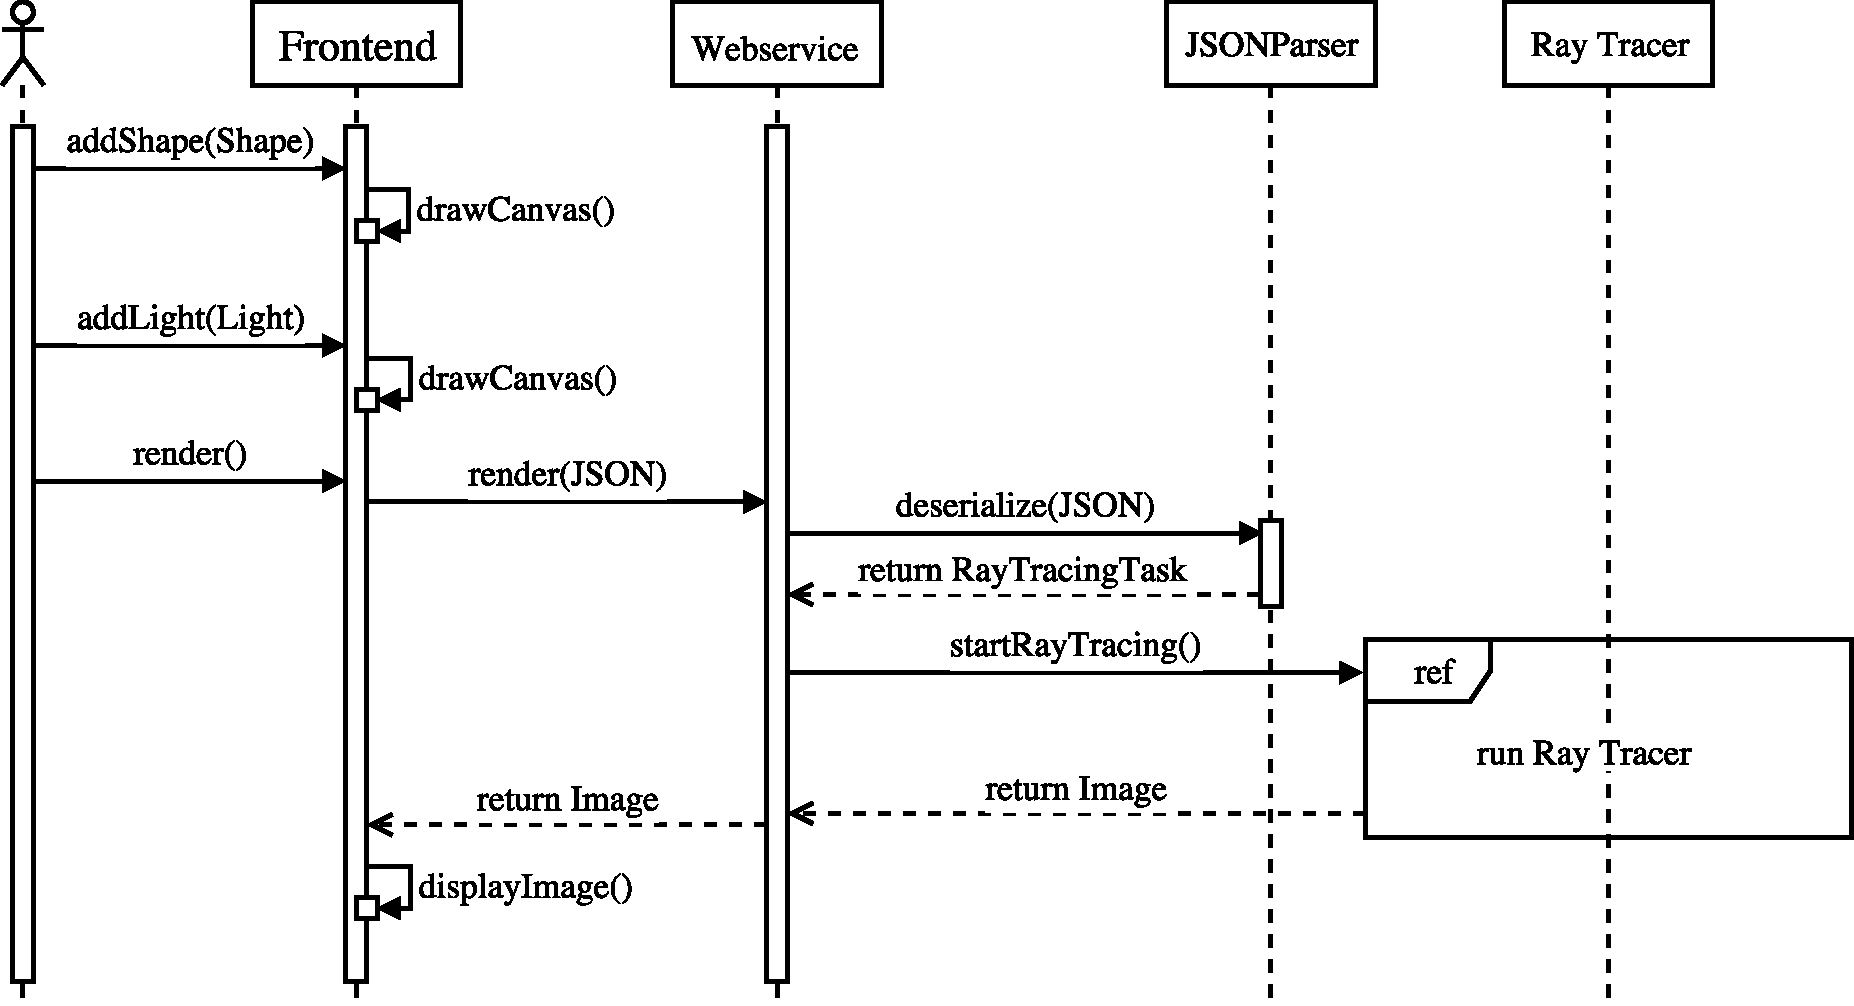
\includegraphics[width=0.8\textwidth]{images/seq_comm.pdf}
  \caption{Sequence-Diagram for the Communication between Frontend and Backend} 
  \label{fig:seqcom} 
\end{figure}

\subsection{Implementation}

\subsubsection{Model}

To provide the required functionality we implemented different classes. A class diagram is attached in the appendix to provide an overview about the classes.

\paragraph{Ray}

A ray in the ray tracer is a line that is described by an origin and a direction point. The equation 

\begin{center}

$ \overrightarrow{V} = \begin{pmatrix} x\textsubscript{O} \\  y\textsubscript{O} \\  z\textsubscript{O} \end{pmatrix} + t * \begin{pmatrix} x\textsubscript{D}  \\ y\textsubscript{D}  \\ z\textsubscript{D} \end{pmatrix}  $

\end{center}

is used to represent it in a three-dimensional room. 

\subsection{Object3D}

The Object3D class is the parent class of all shapes in a ray tracer scene. This relationship is clearly visible in the class diagram. We decided to chose this implementation because each object in the scene can be described by the same default attributes like a center, color, reflection, specular reflection, transparency and refractive index. Also all of the objects provide a method to calculate the intersection with a ray. 

\subsubsection{Sphere}

\paragraph{Intersection}

The intersection of a sphere is easy to calculate. In a three-dimensional room a sphere is described by the following equation, where x\textsubscript{s}, y\textsubscript{s} and z\textsubscript{s} specify the center of the sphere and r represents the radius:

\\
\begin{center}

(x - x\textsubscript{s})\textsuperscript{2} + (y - y\textsubscript{s})\textsuperscript{2} + (z - z\textsubscript{s})\textsuperscript{2} = r

\end{center}
\\

To get the intersection between the ray and the sphere we replace x, y and z by the appropriate lines of the ray equation. We receive the following equation:

\\
\begin{center}

((x\textsubscript{o} + t x\textsubscript{D}) - x\textsubscript{s})\textsuperscript{2} + ((y\textsubscript{o} + t y\textsubscript{D}) - y\textsubscript{s})\textsuperscript{2} + ((z\textsubscript{o} + t z\textsubscript{D}) - z\textsubscript{s})\textsuperscript{2}  = r

\end{center}
\\

Which we can now solve for t. This equation is now solvable by using a quadratic-formula. As a result we receive two values for t - t\textsubscript{1} and t\textsubscript{2}.

We now select the smallest positive t and insert it into the ray equation to receive the point of intersection. 

\paragraph{Surface Normal}

To calculate the surface normal of a sphere we just subtract the center of the sphere from the point of intersection.

\subsubsection{Cube}

A cube is a cuboid just with the same length for all edges. Therefore it is a subclass of the cuboid class, which again is a subclass of the Object3D. At the moment our RayTracer only renders cubes. 

\paragraph{Intersection}

To calculate the intersection with a cube we are using an algorithm that was proposed by Williams et al.. It is an adjusted version of the algorithm that was developed by Brian Smits. Instead of using division Williams et al. suggested to multiply with the inverse. This increases the speed of the calculation which in our case is not considerable but for larger scenes with hundreds of cubes noticeable. 

\paragraph{Surface Normal}

As mentioned for the calculation of reflection, refraction etc. we need the surface normal of the intersection point. For a cuboid there are six different possibilities, one for each of the six surfaces. To get the correct case, we just check which surface was intersected. 

\subsubsection{Cylinder}

The cylinder is a special kind of quadric surfaces. As a quadric surface we understand a polynomial of the order 2 (quadratic). Similar to the sphere we can describe the cylinder by an general equation:

\\
\begin{center}

(x)\textsuperscript{2} + (y)\textsuperscript{2} = r

\end{center}
\\

The z-value does not appear in the equation because the object has a infinite height in the z-direction. For our RayTracer we had to change the equation to 

\\
\begin{center}
(x)\textsuperscript{2} + (z)\textsuperscript{2} = r
\end{center}
\\

because in our scene the y-axis describes the height of the object and the z-axis the depth.

\paragraph{Intersection}

For the intersection with the ray we inserted the ray into the equation of the cylinder and solved for t. Because of the quadratic polynomial we could use the quadratic-formula to solve the equation. Again we received two values  t\textsubscript{1} and t\textsubscript{2}. Because of the infinite height, we always have to check if the point of intersection is between the bottom and the top of the cylinder. Figure \ref{fig:cylinderexmpl} shows an example of the intersection. The problem is that the cylinder is intersected by the ray above the top cap. We now have to calculate another intersection with the top cap of the cylinder to get the second point of intersection. Of course the same could happen to the bottom of the cylinder.

\begin{figure}[h]
  \centering
  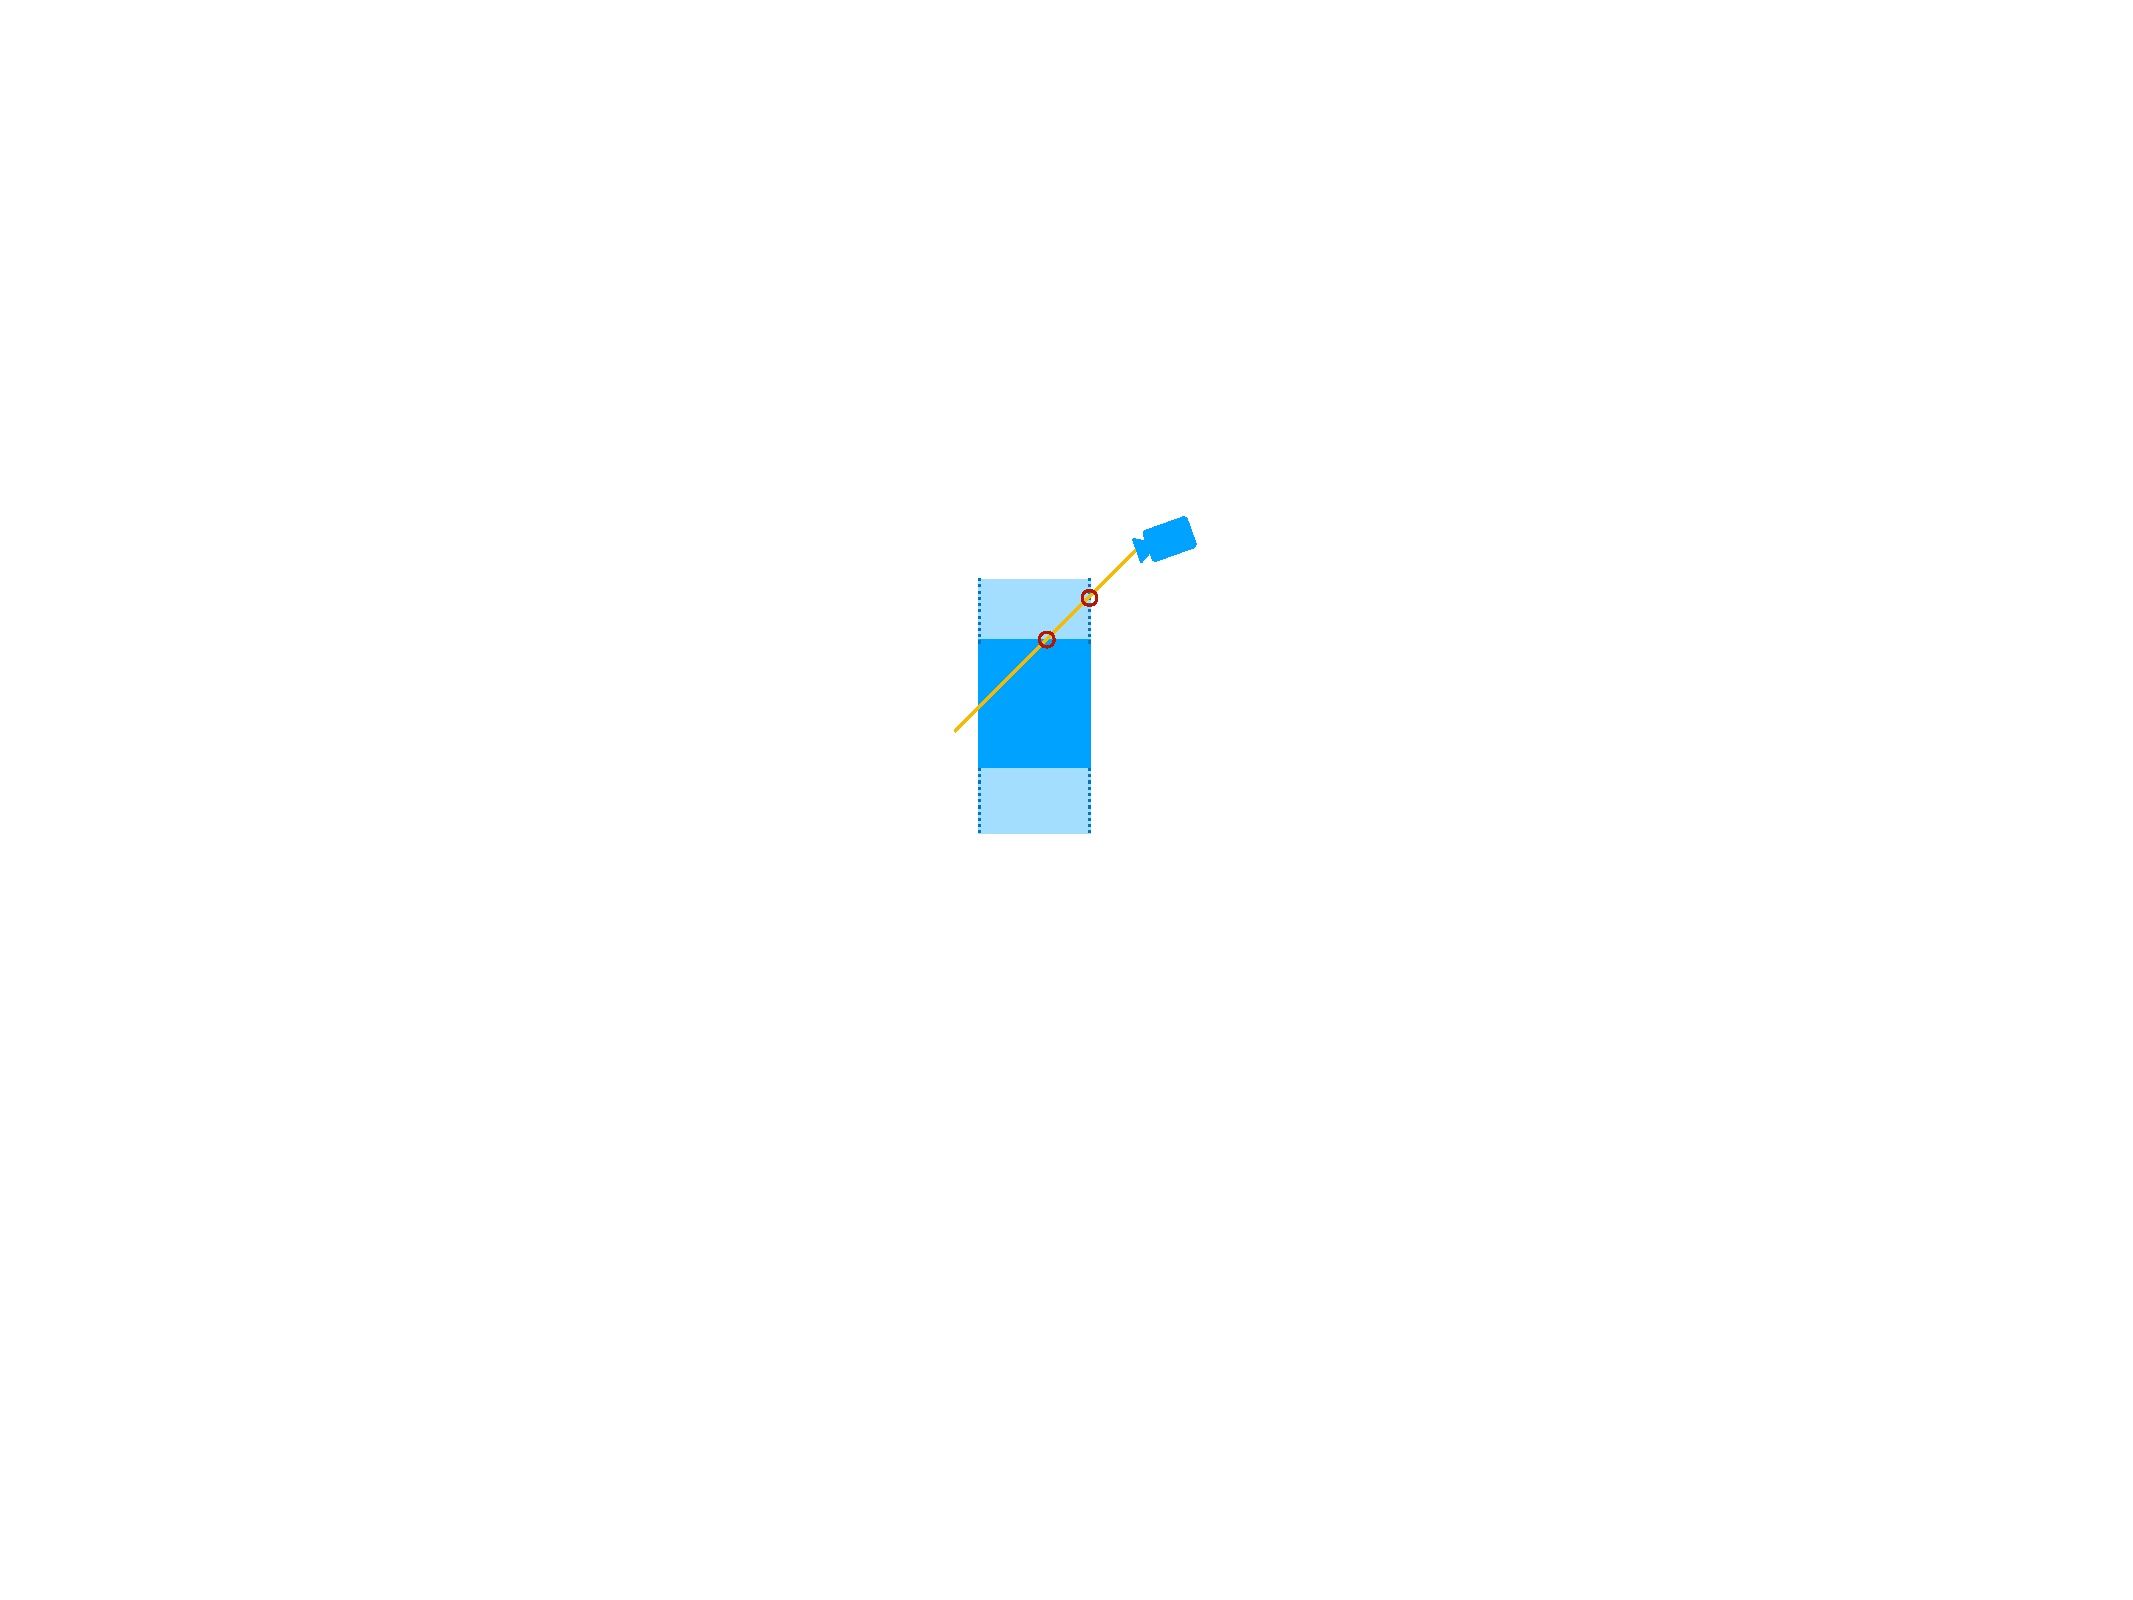
\includegraphics[width=0.2\textwidth]{images/cylinder.pdf}
  \caption{Example of an Intersection with a Cylinder} 
  \label{fig:cylinderexmpl} 
\end{figure}

\paragraph{Surface Normal}

It is a bit more complicated to calculate the surface normal of the cylinder. We first have to differentiate, if the ray hits one of the caps or the surface. If it hits one of the caps we just return the surface normal of the plane. Otherwise we calculate it by subtracting a point v from the point of intersection. The point v in this case is just a point in the central axis of the cylinder at the same y-value of the intersection point.

\subsubsection{Cone}

As the cylinder the cone is a quadric surface with the same attributes than the cylinder. Therefore, cone inherits its attributes from the calls Cylinder.

\paragraph{Intersection}

The intersection for a cone is equal to the intersection of the cylinder. Because of the infinite height, we have to run through the same checks as for the cylinder.

\paragraph{Surface Normal}

The following listing shows the code to calculate the surface normal:

\begin{lstlisting}
def getSurfaceNormal(self,point):

        surfaceNormal = Vector()

        epsilon = 0.00001

        if point.y > self.center.y - epsilon:
            surfaceNormal.y = 1
            return Vector(0.0, 1.0, 0.0)
        elif self.bottom.y - epsilon < point.y < self.bottom.y + epsilon:
            surfaceNormal.y = -1
            return Vector(0.0, -1.0, 0.0)

        x = point.x - self.center.x
        z = point.z - self.center.z

        r = math.sqrt(math.pow(x, 2) + math.pow(z, 2))
        surfaceNormal = Vector(x, r * (self.radius / self.height), z)
        return surfaceNormal.normalize()
\end{lstlisting}

\subsection{Parallel Processing}

Because of the enormous number of calculations during the rendering process and the relating performance issues we decided to implement multiprocessing. The rendering task is a perfect use case for it because each pixel of the final image is calculated independently from the other pixels. 

\subsubsection{Multithreading in Python}

The first attempt was to use multithreading to parallelize the raytracing task. But in Python multithreading works differently. During the execution of a Python program only one interpreter is used and executed. That means even if we run multiple threads, only one thread is executed at the same time and the other threads are locked by the Global Interpreter Lock (GIL) and have to wait until the interpreter is free. Because of this limitation a real parallelization was not possible and we had to find another way for our implementation. 

\subsubsection{Multiprocessing in Python}

Because of the constraints of multithreading we implemented multiprocessing. Instead of just creating multiple threads Python creates complete new standalone child processes. These processes are forked from the parent process and therefore have the same attributes. In \ref{fig:processhierarchy} we can see the hierarchy of the processes and the different process ids. 

\begin{figure}[h]
  \centering
  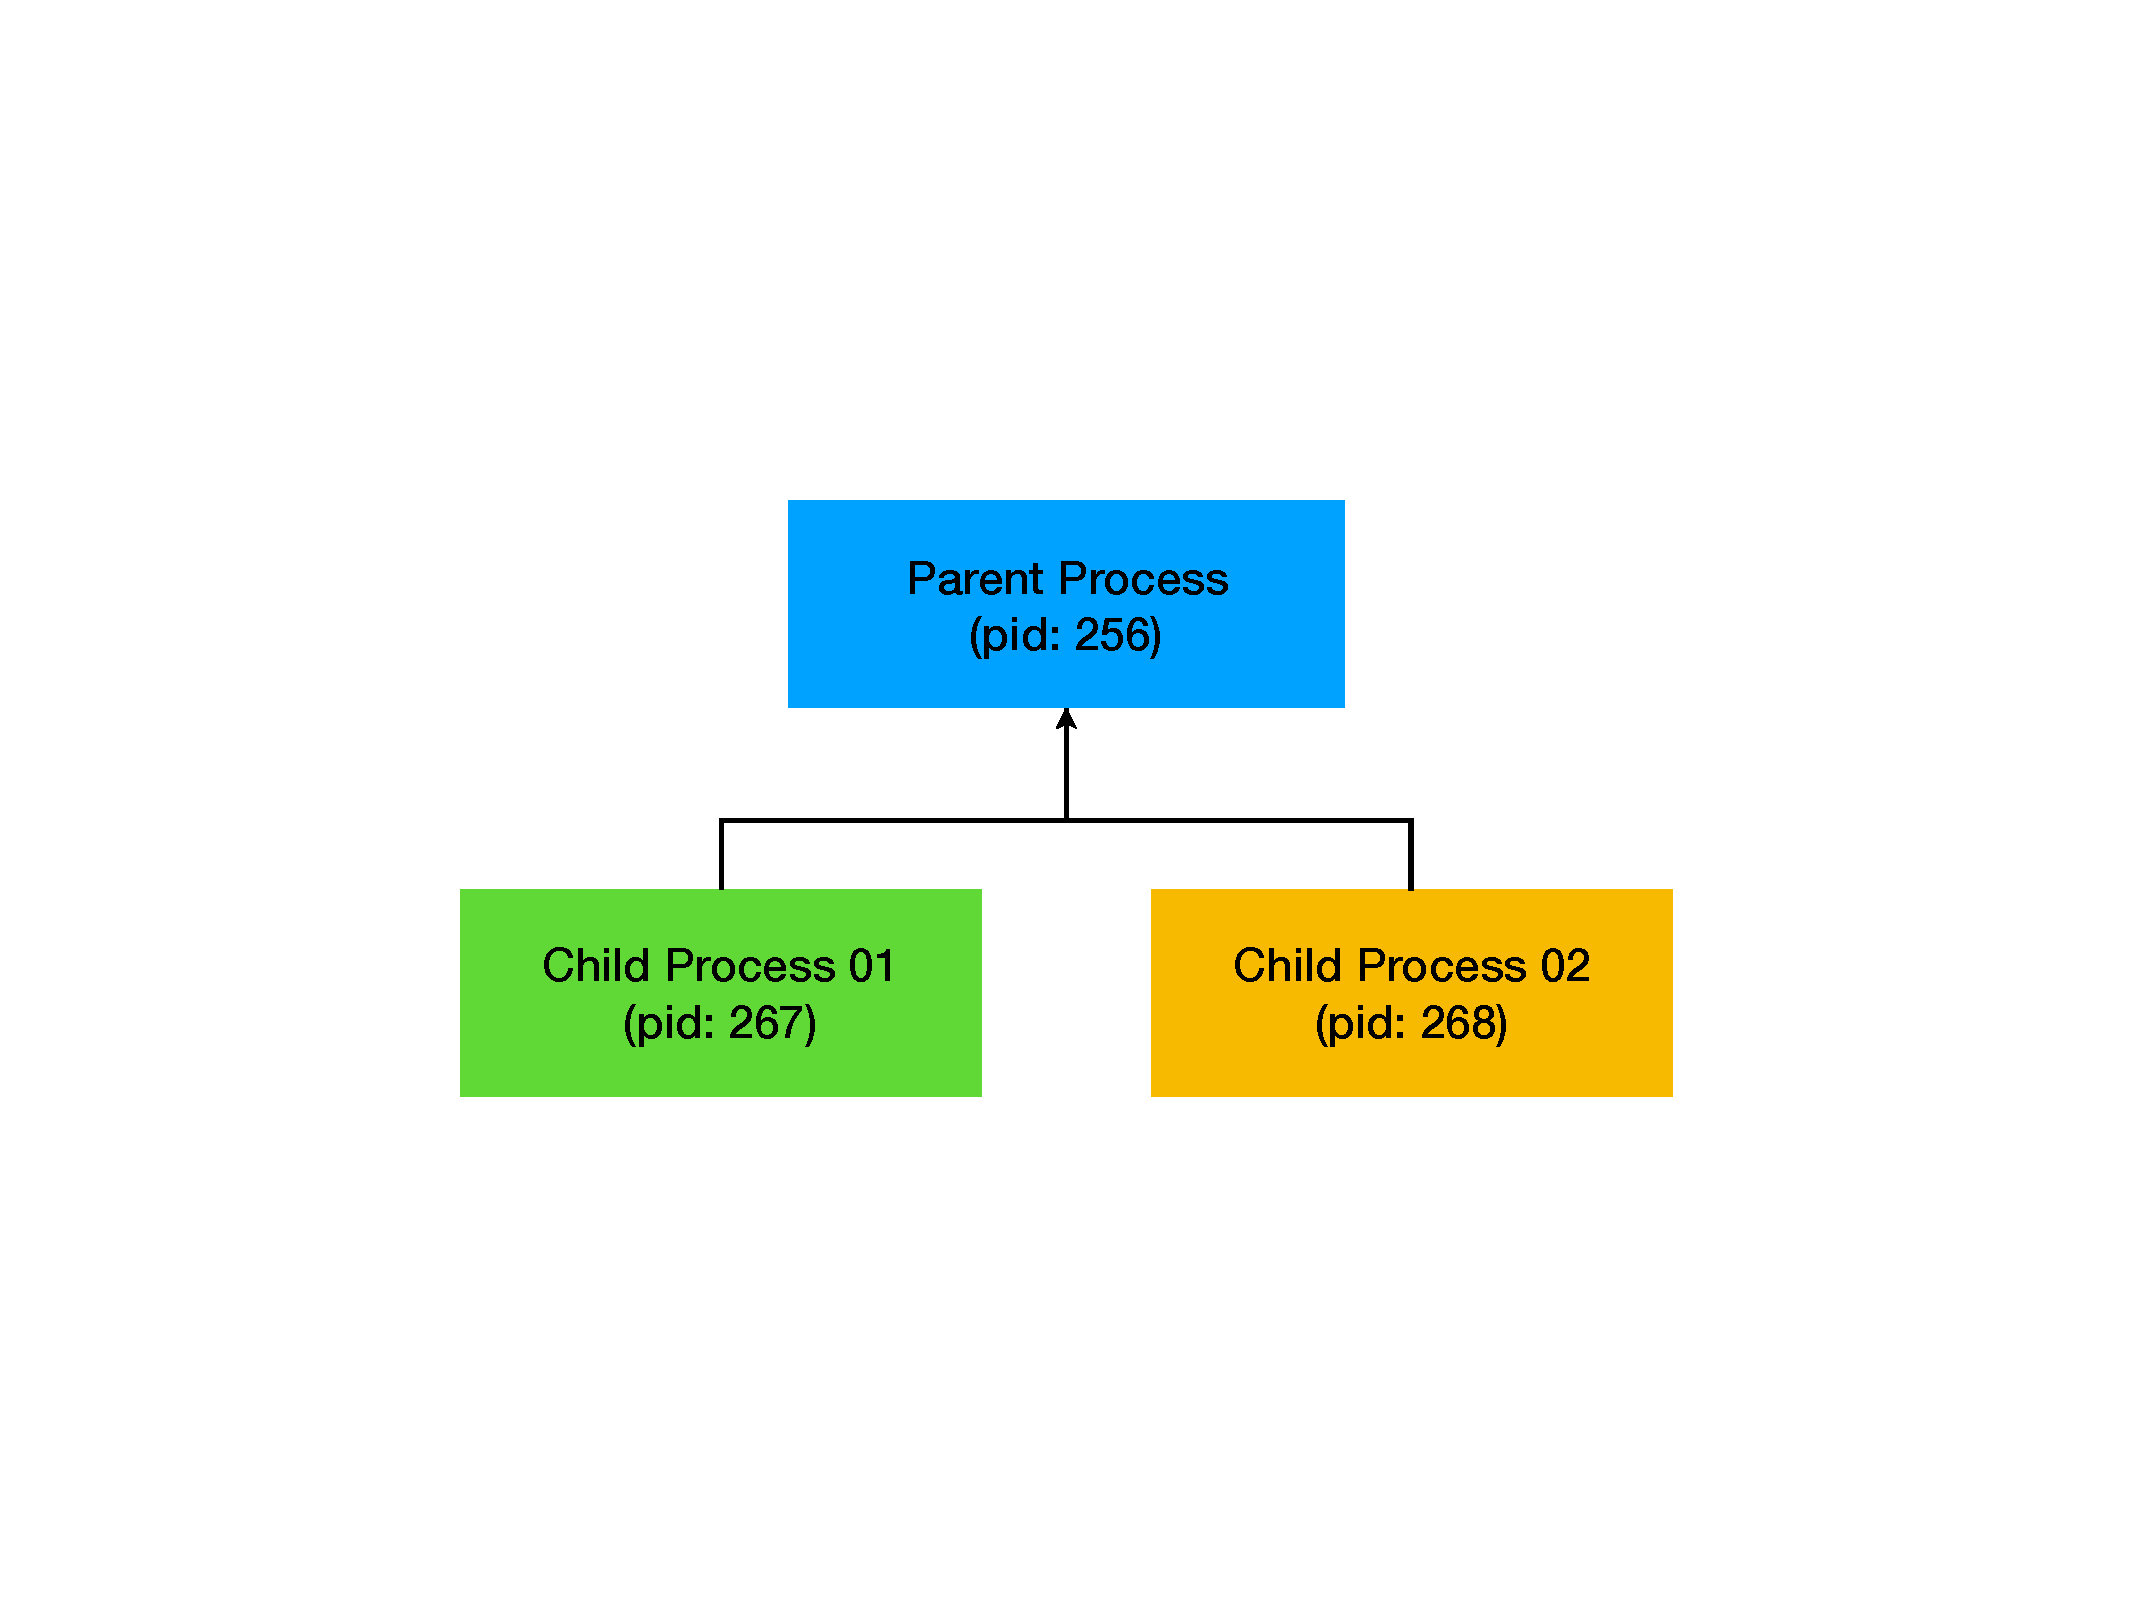
\includegraphics[width=0.4\textwidth]{images/processhierarchy.pdf}
  \caption{Process Hierarchy} 
  \label{fig:processhierarchy} 
\end{figure}

One of the most critical disadvantages are the separated memory spaces. Each process has its own memory space and is unable to access the memory of other processes. The parent process is unable to access the attributes of his child processes and the other way round (see figure \ref{fig:memory}). There are to ways to circumvent this limitation. 

\begin{figure}[h]
  \centering
  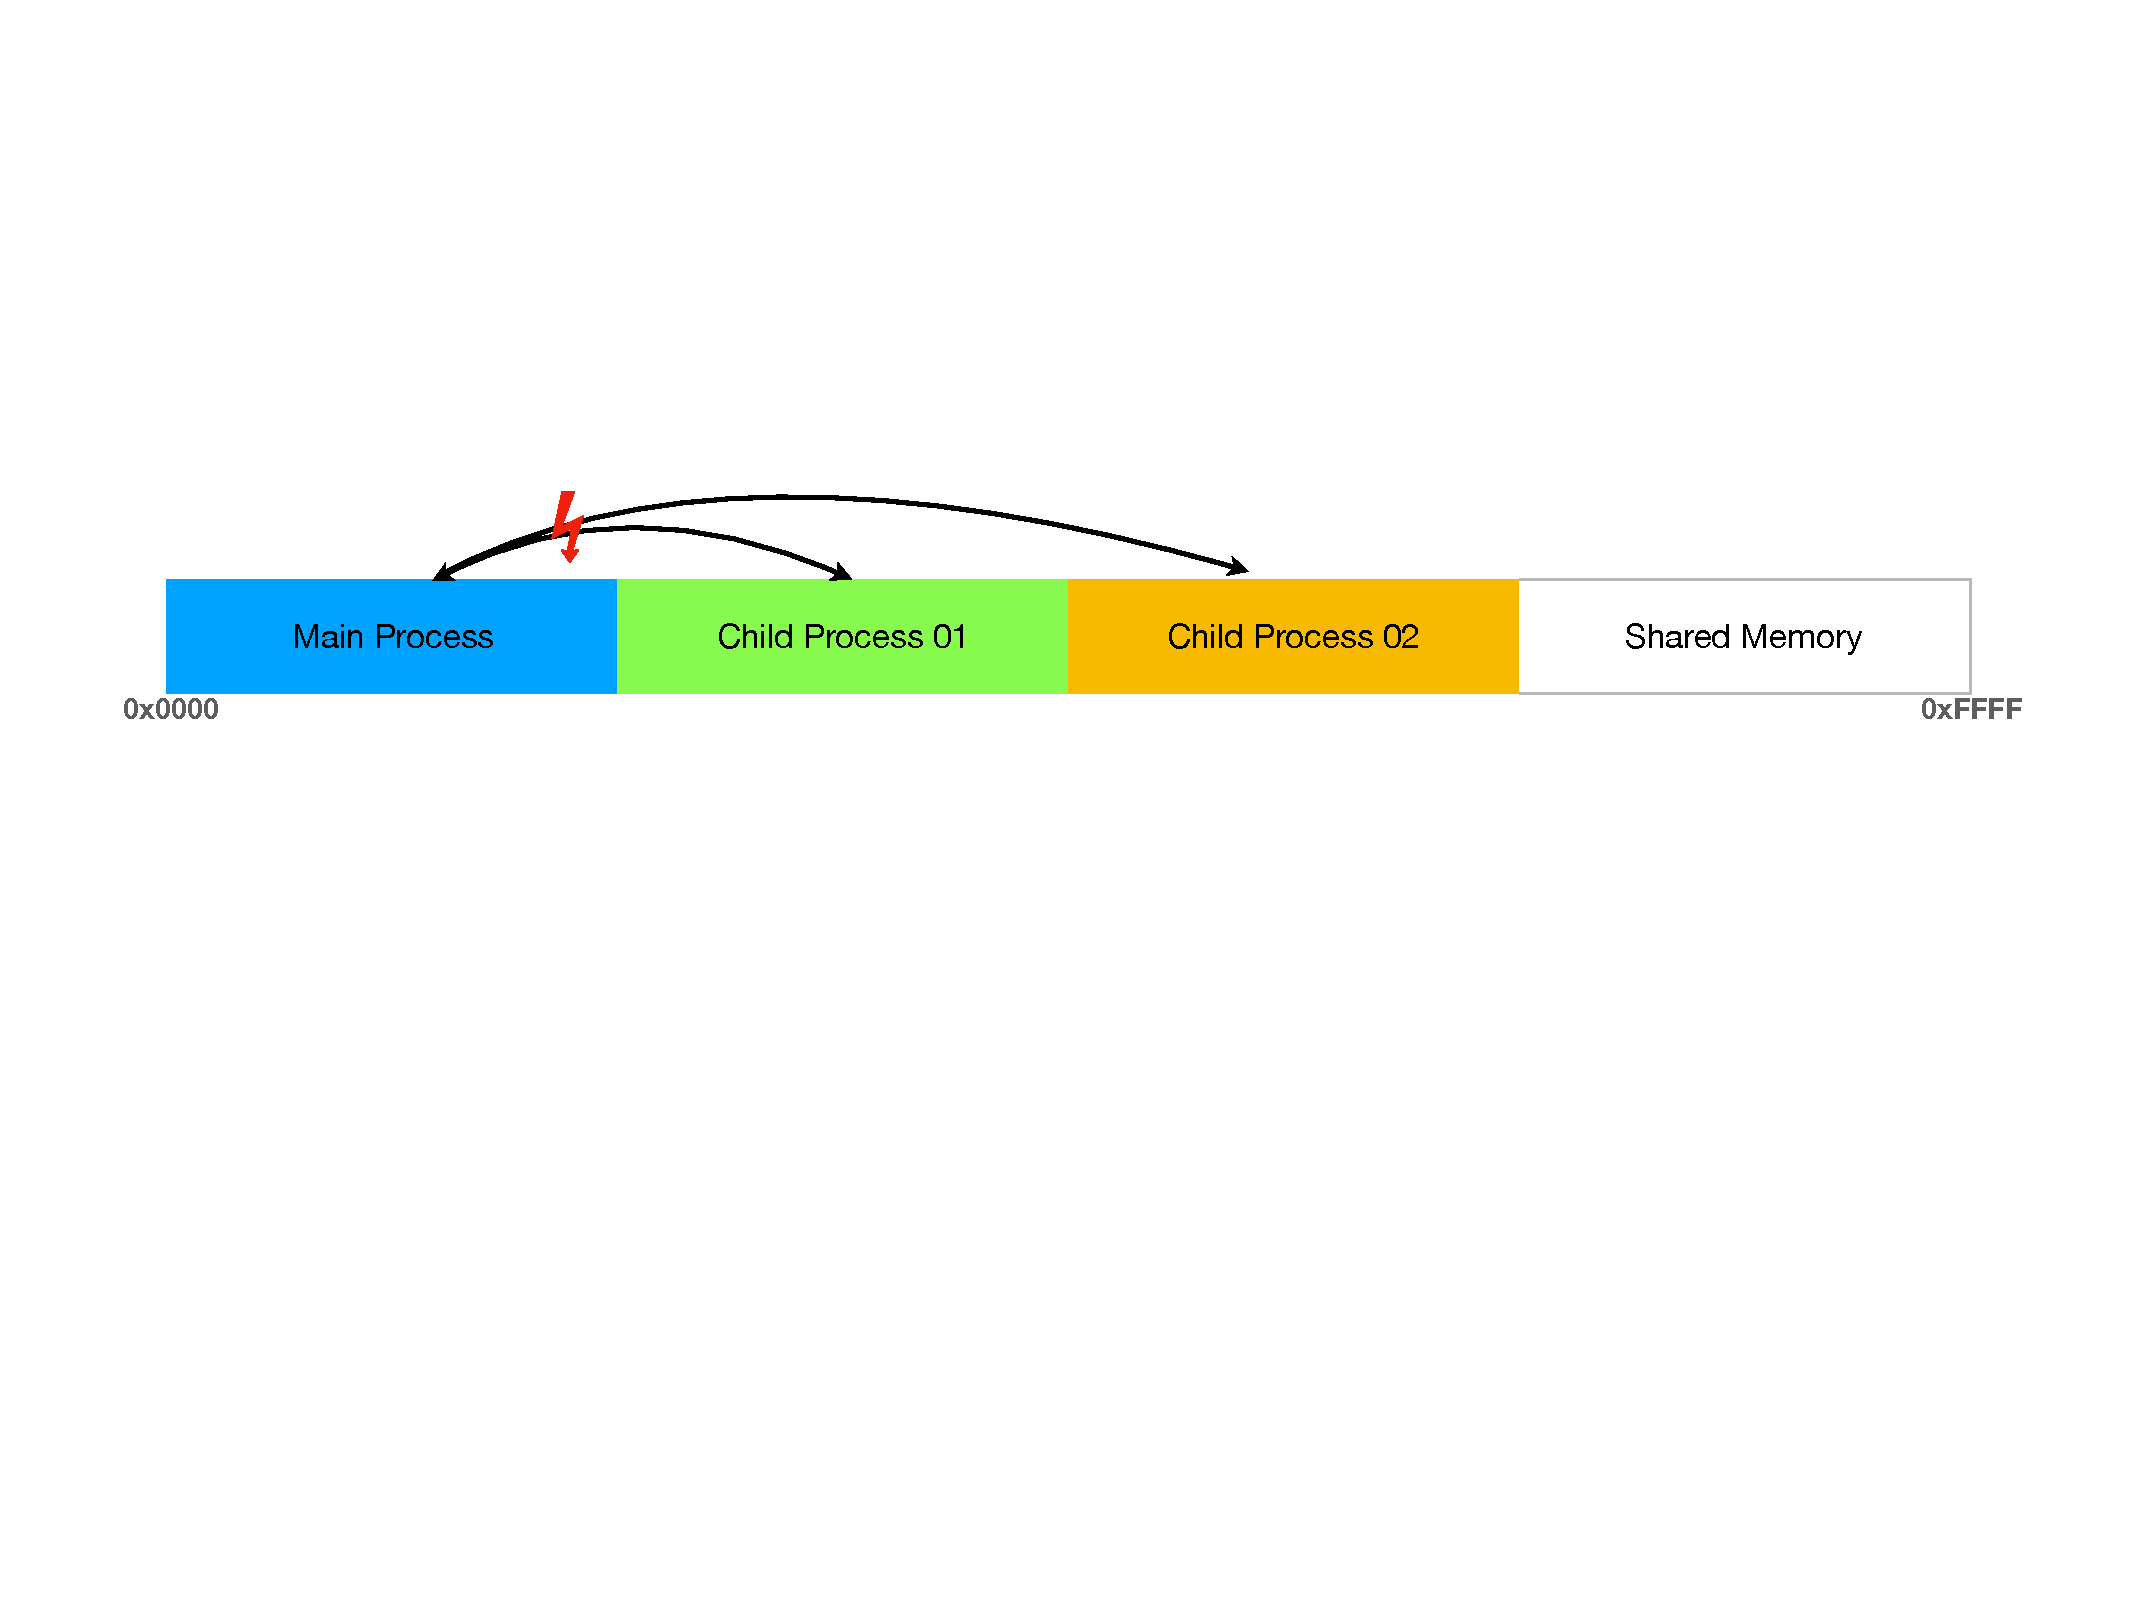
\includegraphics[width=\textwidth]{images/memory.pdf}
  \caption{Memory allocation of processes} 
  \label{fig:memory} 
\end{figure}

\paragraph{Shared Memory}

We could allocate memory space that is shared by the parent and child process. If we now store for example an integer in this memory it is read- and writeable from both processes. By default Python provides the possibility to store an array, double and integer values in the shared memory. Unfortunately, complex objects could not be stored with this method. In our case we wanted to store a multidimensional array that represents the pixels of the image.

\paragraph{Base Manager}

Another possibility to share objects between the processes is the so-called Base Manager. Managers provide a way to create data which can be shared between different processes. A manager object controls a server process which manages the shared objects. Other processes can access the shared objects by using proxies \cite{pythondocu}.

\subsubsection{Implementation}

We implemented the parallelization by splitting the scene into equally sized parts as shown in image \ref{fig:processsplit}. This is an example for a scene with the size of 500 x 500 pixels on a computer with a 4-core CPU. With this technique and multiprocessing we could fully parallelize the ray tracer and increase the rendering speed by almost the factor 4. Figure \ref{fig:renderingcmp} shows the rendering time of the image \ref{fig:exmplscene} with 1, 2, 4 and 8 cores. 

\begin{figure}[h]
  \centering
  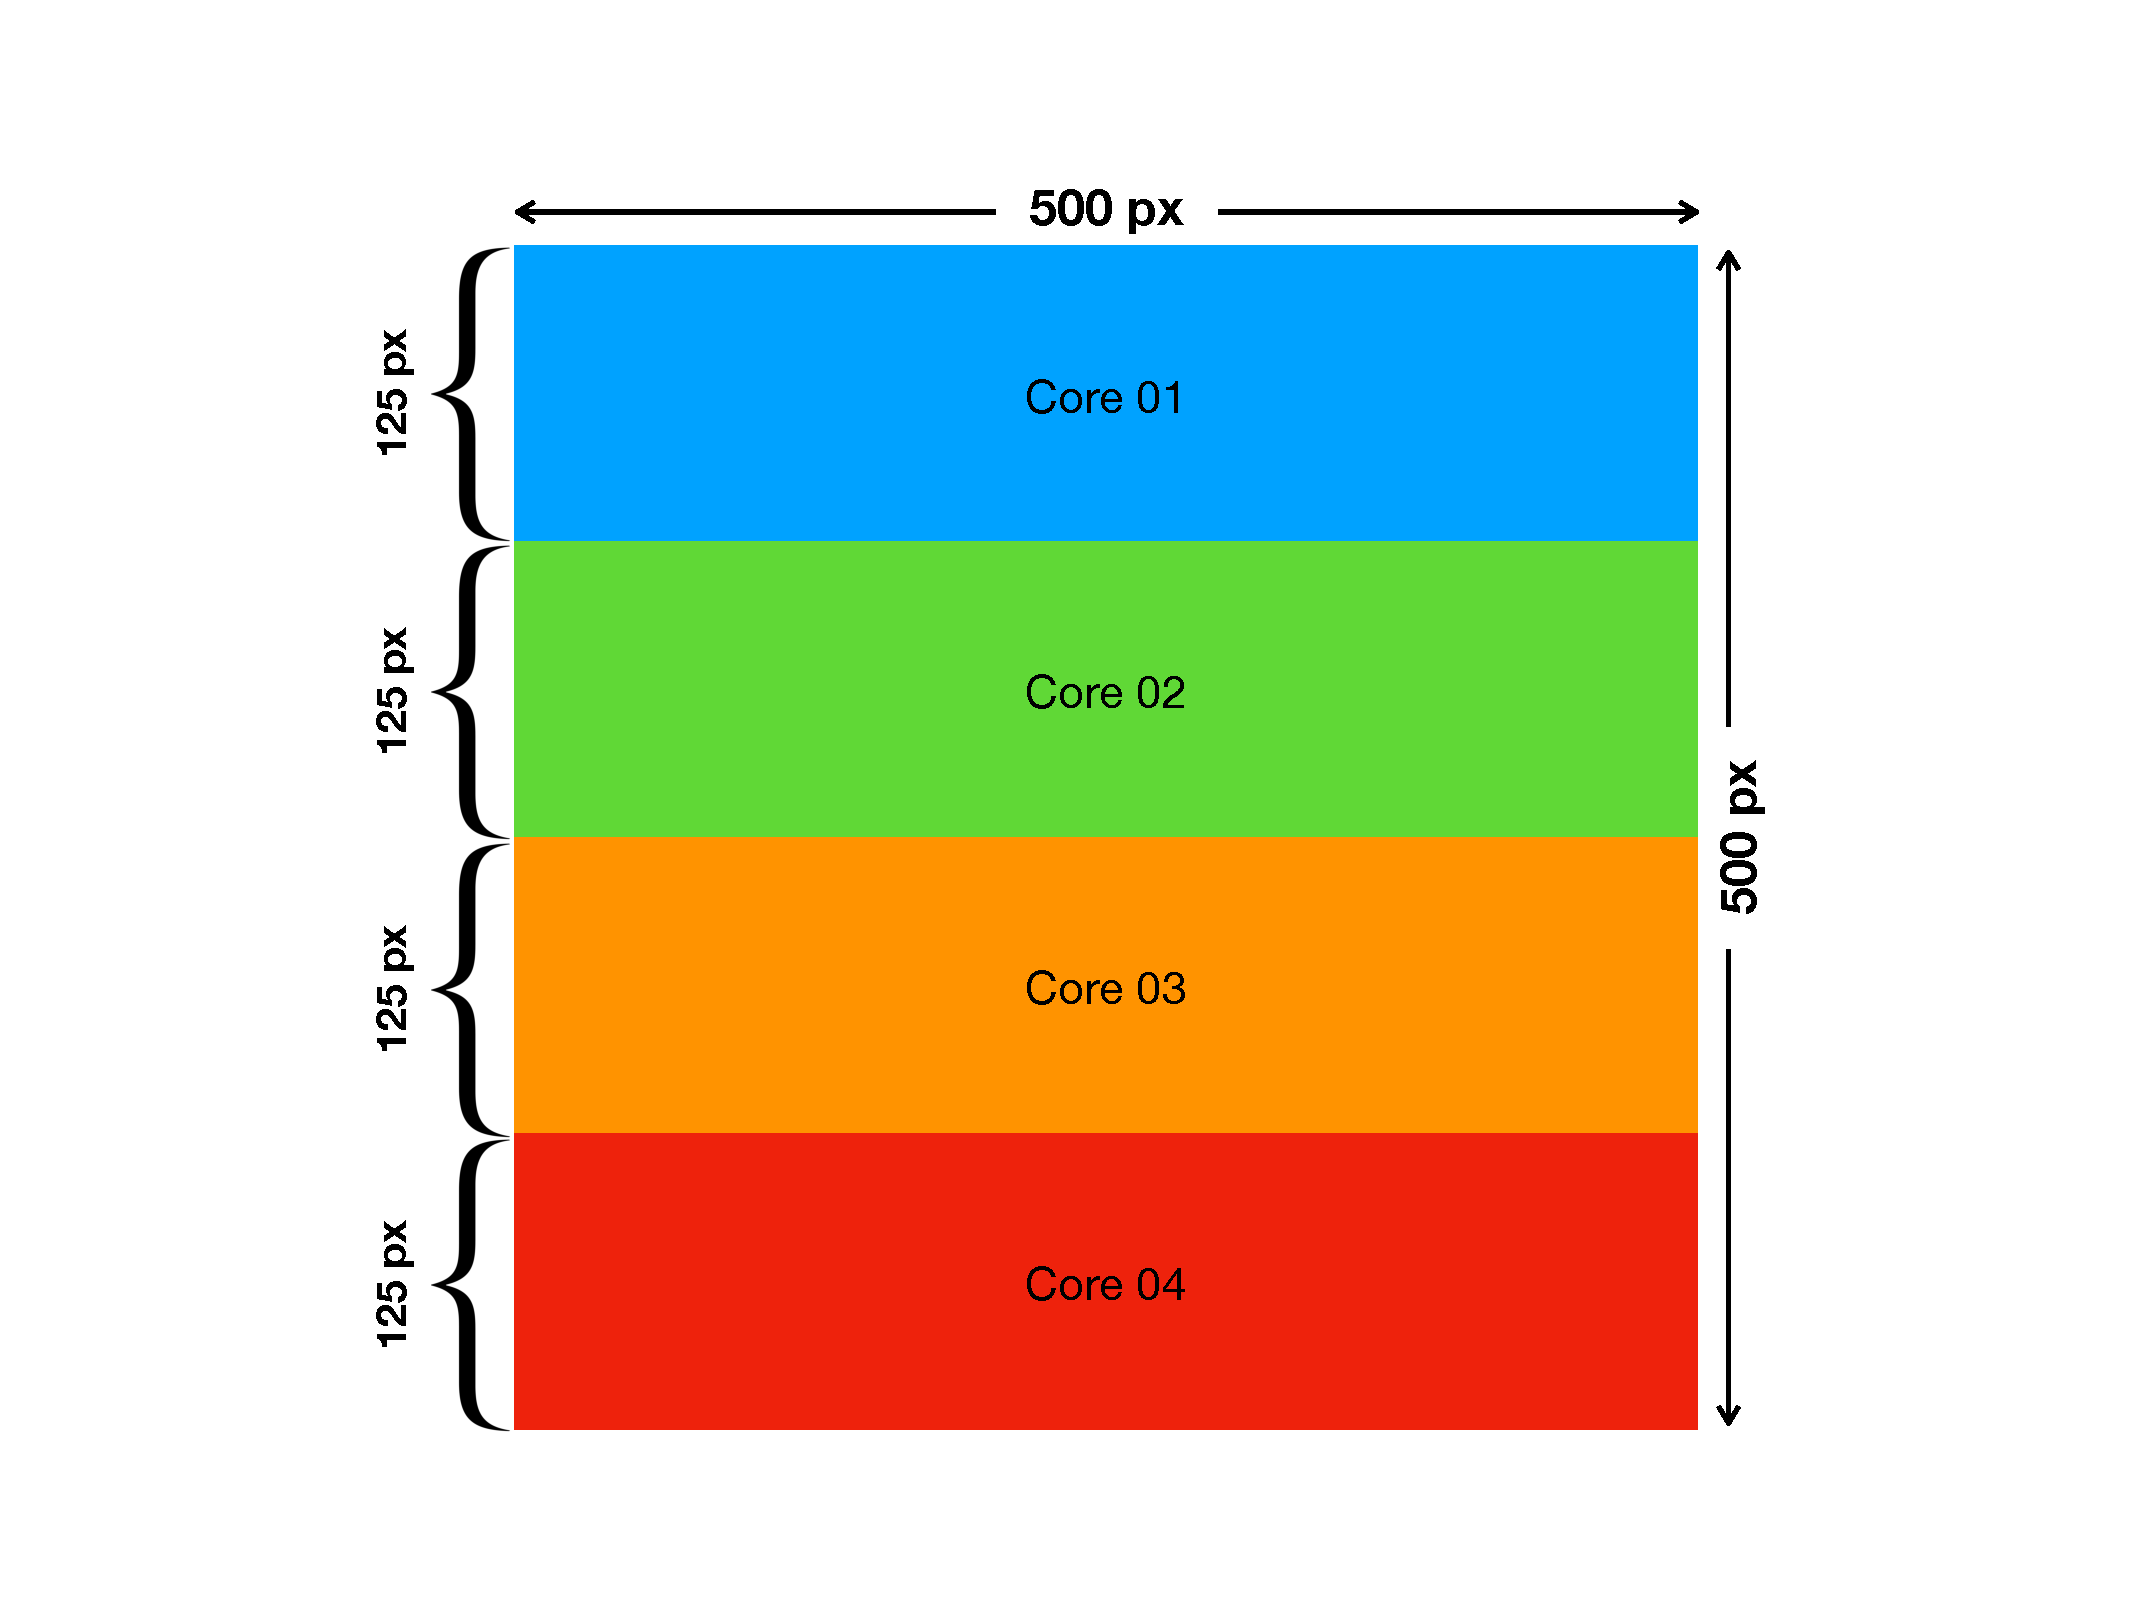
\includegraphics[width=0.6\textwidth]{images/processsplit.pdf}
  \caption{Example of splitting the work} 
  \label{fig:processsplit} 
\end{figure}

\begin{figure}[h]
  \centering
  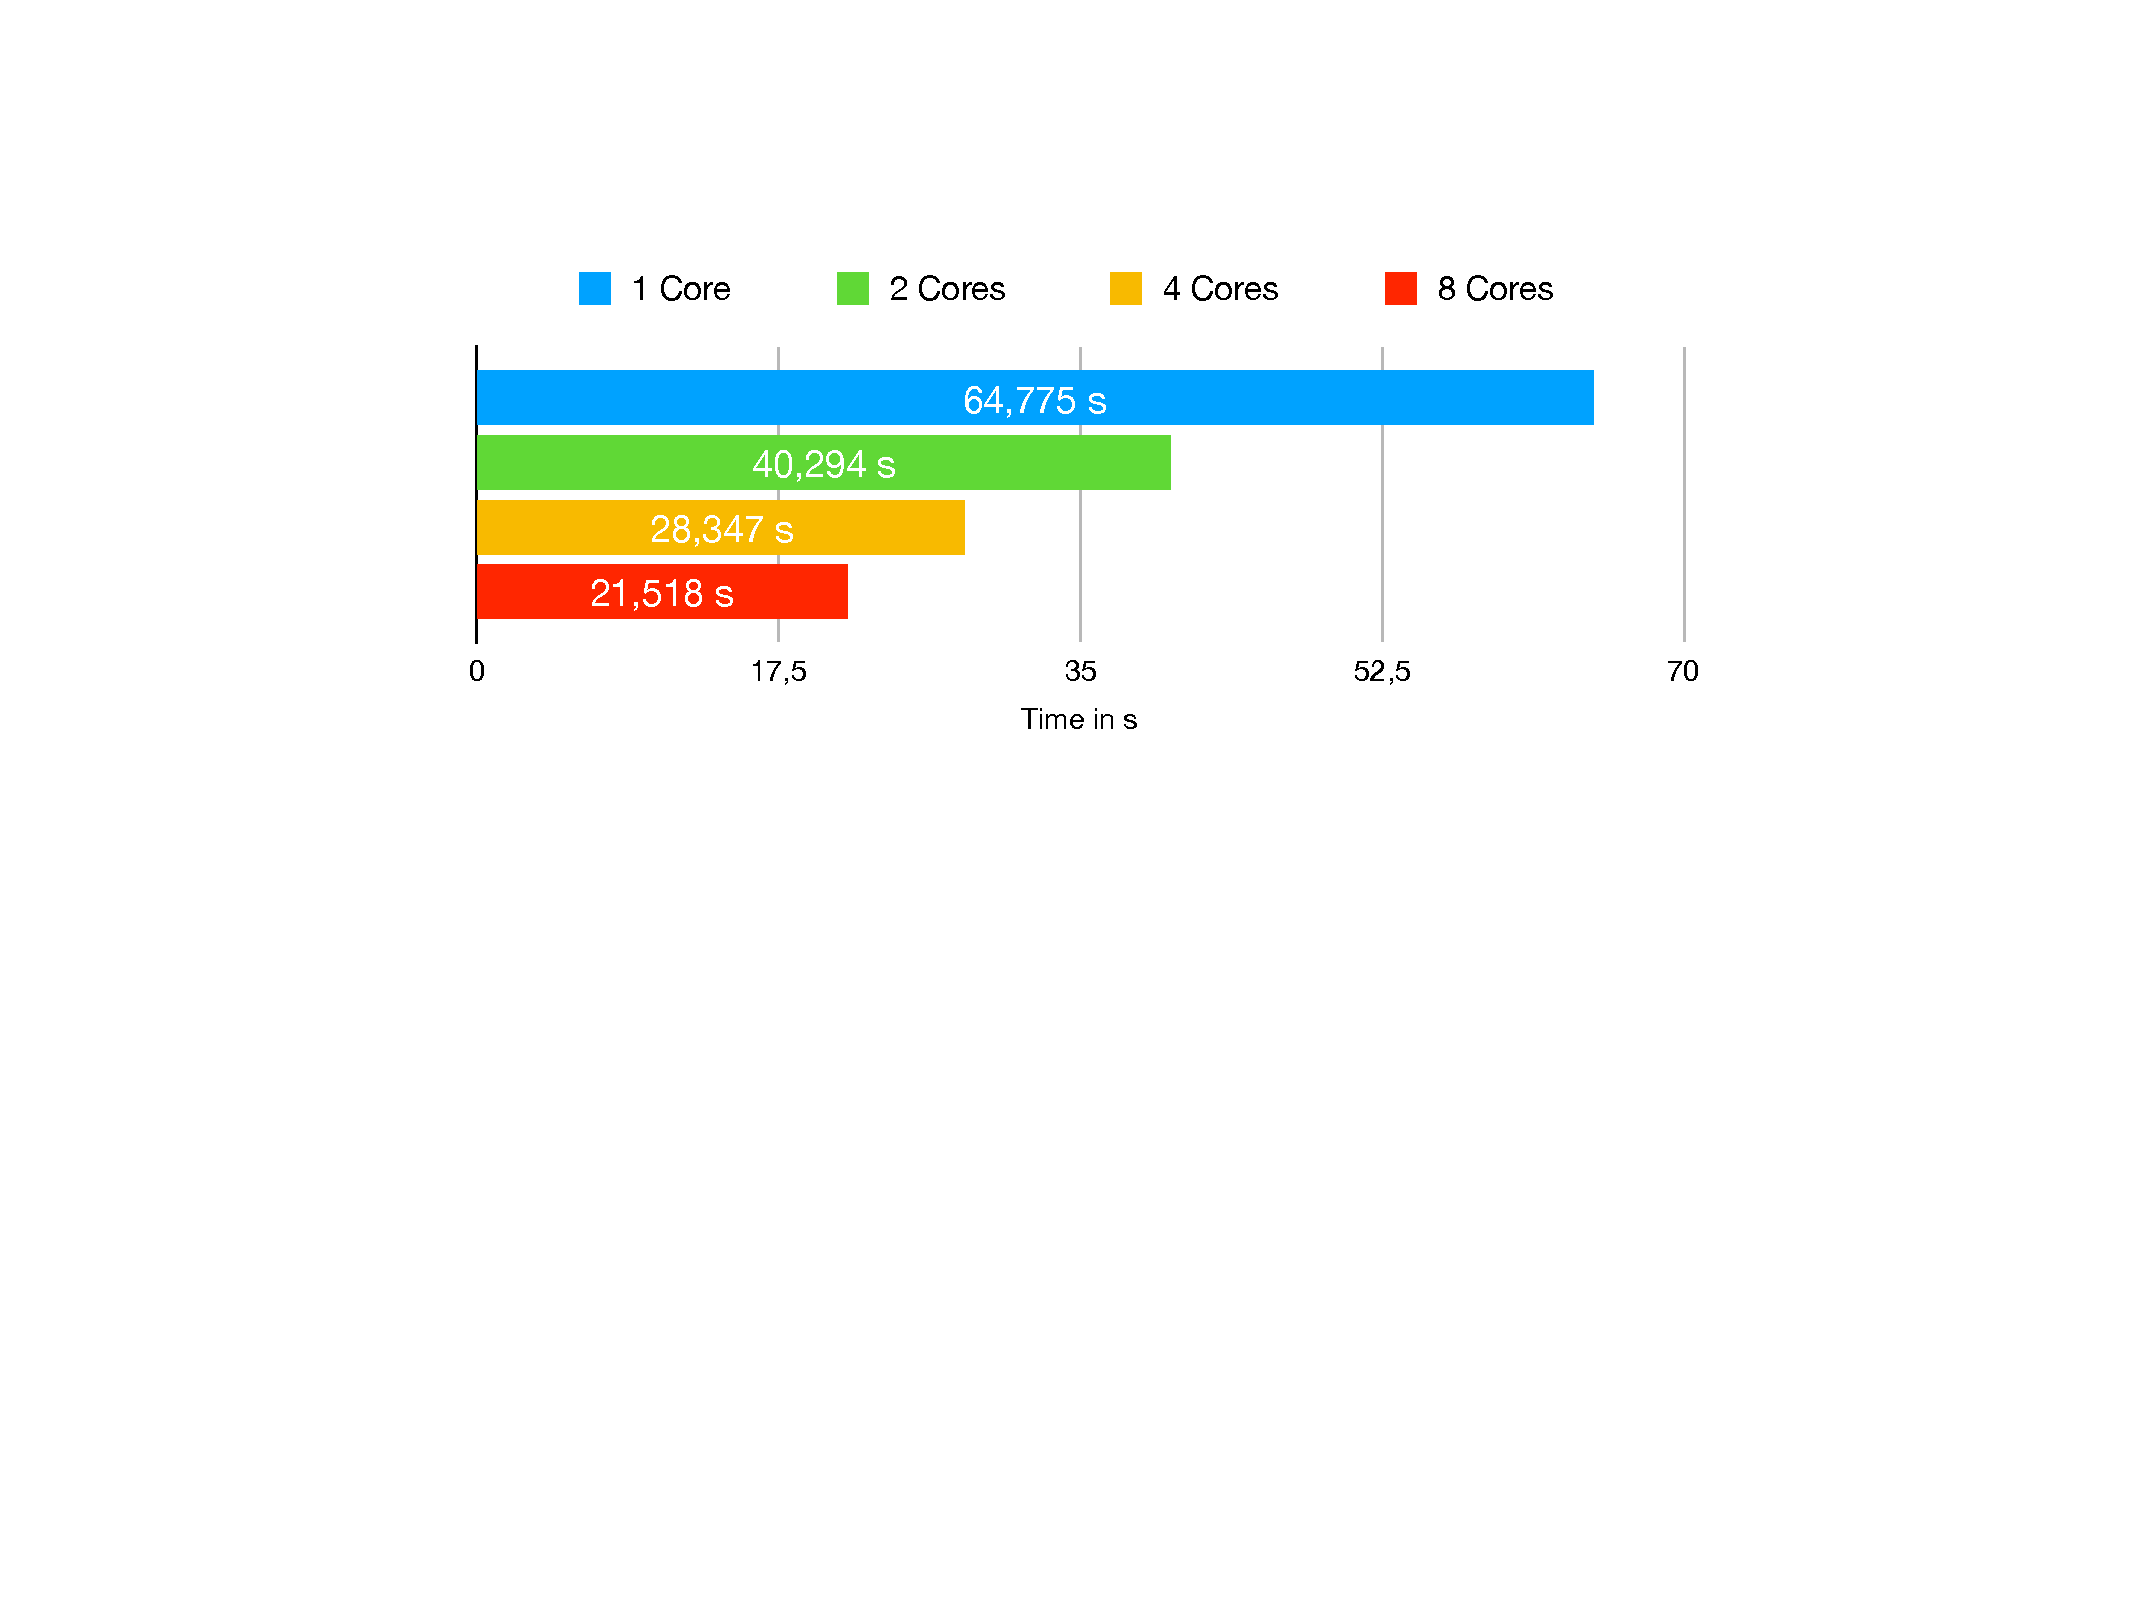
\includegraphics[width=0.8\textwidth]{images/renderingcmp.pdf}
  \caption{Performance comparison of mutliprocessing} 
  \label{fig:renderingcmp} 
\end{figure}

\begin{figure}[h]
  \centering
  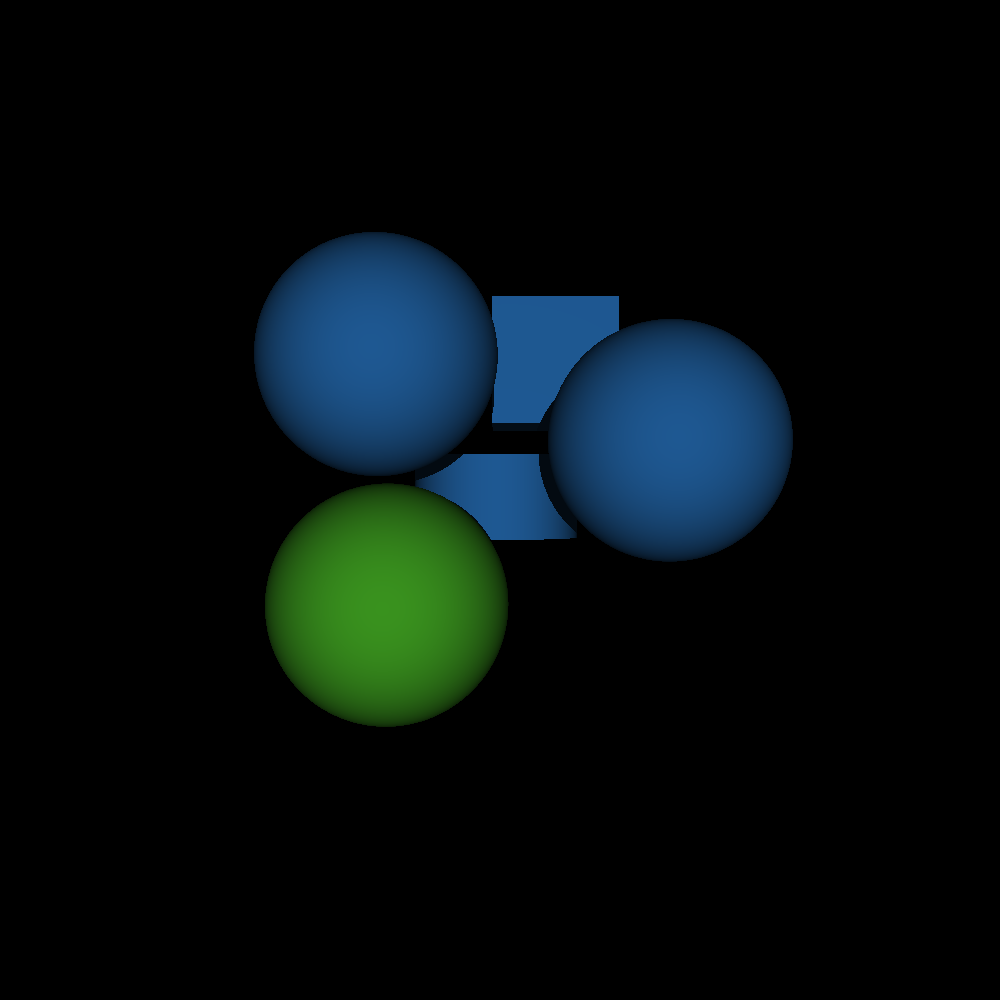
\includegraphics[width=0.4\textwidth]{images/exmplscene.png}
  \caption{The rendered image from the benchmark} 
  \label{fig:exmplscene} 
\end{figure}

\subsection{Implementation of Ray Tracing}

In order to implement the ray tracer we read a lot of tutorials and articles online.
Mainly we based our code in this tutorial \cite{gambriel}
and this online lessons \cite{scratchaPix}.

\subsubsection{Pixels}
To start the ray tracer, we essentially have to "position" the frame in front of the camera. In reality, there is no actual frame, we just use the position and direction of the camera to first calculate where our rays should be directed towards. Then for each pixel of the image, depending on what the user defined, we sent out a ray to calculate the color of pixel. In the function trace() for each pixel we calculate the x (pixelX) and y (pixelY) of the direction that the Ray has to take to calculate the color for each pixel. The calculations are shown below.

\begin{lstlisting}
    pixelX = 2 * x / self.imageplane.getWidth() - 1
    pixelY = 1 - 2 * y / self.imageplane.getHeight()

    pixelRay = self.camera.getRay(pixelX, pixelY)
\end{lstlisting}

To explain the code let's take for example an image of 100x100. At first we calculate pixel (0, 0) which will have a direction of (-1,1). The second pixel of the image (1,0), will have the direction (-0.98, 1). We repeat the process until we place every pixel of the image on our space. Of course, this example is extremely simplified, in reality we are dealing with 3D space so those calculated pixels have to be placed in a 3D space. For example, in the case our camera is at (0, 0, 0) and the direction we are looking towards is (0,0,1), the 3D coordinates of the direction for each pixel ray will be from (-1, 1, 1) to (1, -1, 1). Depending on the position, direction and rotation of the camera we have to change the direction of the ray we are casting, since the starting positions of the rays will always be the position of the camera. These calculations are explained more indepth in the Camera Section.
\par

\subsubsection{Trace Single Ray}
After we have calculated our ray for a pixel we call the function traceRay(), which checks if a ray intersects any object in the scene and returns the closest object that the ray intersects. The only thing to note in this function is this line:

\begin{lstlisting}
for obj in self.scene.getObjects():
    objIntersection = obj.intersection(pixelRay, 0.0001, math.inf)       
\end{lstlisting}

In the above code, we check if there is an intersection with the ray and each object in the scene. The function intersection(), that each Object3D has, takes 3 parameters: the ray we want to check for intersection and two float numbers tMix, tMax. tMin and tMax have to be specified so that the only intersection that can be found is in that distance. In the case of traceRay() we would like to locate items that are in front of the camera only, therefore we ignore intersections that have negative distance from our ray's starting point. Since the ray has a direction, if an intersection is found in the opposite direction it will have a negative distance from our starting point. Finally, if no intersection can be found then we return the color of our background, which is by default black. If an intersection is found, then we call the function getColorForIntersection() with the intersection located as an argument.
\par

\subsubsection{ Color of a single point }
The function getColorForIntersection() computes the color of a certain point. Firstly, it iterates through the Lights to calculate how bright this point is. We add the brightness of the AmbientLight, which is essentially a global light that illuminates everything evenly, and of any other Light that is visible from that point. 

\subsubsection{ Shadows }
\par To find out which Lights are visible from a certain point we run the function getShadows(). What get shadows does is fairly similar to what traceRay() does. It accepts as parameter an Intersection and a Light, from that it calculates a Ray with the point of intersection as a starting point and the position of the Light as a direction. Then it looks if there is any intersection of this ray and any other object in the scene. It has to be noted that here the code to locate an intersection is adapted to:
\begin{lstlisting}
    shadowIntersection = objectIter.intersection(lightToPoint, 0.001, 0.9999)
\end{lstlisting}

We change the value of tMin and tMax because we want to locate only intersections between those two points. If an object intersects our ray beyond these two points we do not care, since it will not cast a shadow on our point. One could note that we are looking for intersections in the range 0 to 1, so what are the small variations for? We change 0 to 0.001 and 1 to 0.9999 so that we ignore any intersection with the object the point is on. Finally getShadows() returns a value for the least transparent object that was found to intersect the ray. That is because if we encounter a solid object then we would like to have complete shadow, while if there is a semi-transparent object between our point and the light it would cast a softer shadow on the point by letting some of the light through. If no intersection is found then we return None.
\par

\subsubsection{ Diffuse Reflection and Specular Reflection }

After getColorForIntersection receives the return value from getShadows() it can calculate how much the point is lit from each Light. To do that it calls a function called diffuseAndSpecularReflection(). This function calculates how bright a specific point is based on the position of a specific light. This is done in this part of the function:

\begin{lstlisting}
    surfNormDotLTP = surfaceNormal.dotProduct(lightToPoint)
    if surfNormDotLTP > 0:
        colorBrightness += light.getBrightness() * surfNormDotLTP / lightToPoint.calcLength()
\end{lstlisting}

It works in the following way: we calculate the dotProduct of the Vector of our ray from the light to the point and the surfaceNormal of the object at the point of intersection. For example, if this point is in the back of an object then this dotProduct will be negative and it would not be illuminated at all. As we can see if the dotProduct is bigger than 0 then we perform a calculation based on the angle that the light and the surfaceNormal are (using the same dotProduct) and the distance of the light from the object to calculate how much light that specific point should receive. This is what we call diffuse reflection. Then the function diffuseAndSpecularReflection, also calculates specular reflection for the specific point. Each object has a degree of specularity, which essentially indicates how shiny an object is. Following a bit more complicated calculations than for diffuse reflection, we can calculate how much more light some points must get, based on the specularity of the object and the angle of the light to the surface normal of the object at the specific point. Then the brightness of the light is returned to getColorForIntersection().

\par 

\subsubsection{ Reflection }

Using the above information for how each light illuminates the point getColorForIntersection() sums the brightness from each light and calculates the total brightness that a point receives. Consecutively, the function getReflection() is called. If the object that the point is on is not at all reflective then this function returns None. Otherwise, it creates a reflected ray from the object to a new direction. This new direction is calculated using the original direction of the ray and the surface normal of the object at that point. After the new direction is calculated we cast a new ray from the point of intersection towards the new direction and we call again traceRay(). This essentially starts the whole process again from the beginning with a new ray and returns a color based on what this ray intersects. The calculated reflected color gets returned to getColorForIntersection.
\par

\subsubsection{ Refraction }
Afterwards, getColorForIntersection calls the function getRefraction(). This function is fairly similar to getReflection(). If the object the point is on is not at all transparent then it returns None. Otherwise, it will calculate a new ray direction and will call traceRay() to follow said ray and calculate the refracted color, similarly to how getReflection() does. The difference is that this time the new ray will be directed inside the object since our object is transparent. This direction is calculated using the original direction of the ray, the surface normal at the point and the refractive index of the object. The refractive index is a number larger than 1 and shows how refractive the object is. In the real world, different materials have different refractive indices. The refractive index indicates how light propagates through the object. For example, air has a refractive index of 1.000293 and water has one of 1.33 . What this means is that when you are looking through the air you see the positions of the objects accurately, while if you are looking through water the positions of the objects you see get distorted. This happens because when a light ray enters water it changes direction. How much the direction changes depends on the refractive index of a material. In our project, we have a set of refractive indexes that the user can choose from the front end ranging from 1 to 3.4. Finally after traceRay() returns the value of the refracted color, getRefraction sends this value back to getColorForIntersection.
\par

\subsubsection{ Recursive Ray Tracing }
At this point it is good to note that getReflection() and getRefraction() makes our algorithm recursive. A ray can create more rays, that can create more rays depending on how many reflective and refractive objects we have in a Scene. Of course, this would run forever if the scene was full of mirrors. In order to avoid that traceRay() and all subsequent functions keep track of a recursionDepth. We have a recursion limit set to 3, which means that after we have called traceRay() 3 times from the same original ray, then getReflection() and getRefraction() will not call it again and will just return None. We believe than having a recursion limit of 3 is ideal, you can still see 3 reflections on a reflective object and it keeps the run time of the ray tracer to an acceptable level. 

\par

\subsubsection{ Calculation of Final Color }
Finally, after getColorForIntersection has the brightness, the original color, the reflected color and the refracted color, it can calculate the final color of the point. The calculation for the color is done in the following way: if the object is neither reflective nor transparent then it just multiplies the color of the object and the brightness. If it is only reflective or only transparent by a certain degree then the reflected/refracted color is multiplied by the degree of reflectivity/transparency of the object and the original color is multiplied by the inverse rate of that. Reflectivity and transparency can range from 0.0 to 1.0. So the inverse rate would be 1.0 - reflectivity/transparency.
In case the object is both reflective and transparent then if the sum of reflectivity and transparency is 1 ( it will never be more than one because a check is in place to adjust these values in Object3D called checkReflectionAndTransparencyLimit() ) we ignore the original color and just multiply each color with its rate and add them. In case that the sum of reflectivity and transparency is less than 1 then again reflected and refracted colors are multiplied by their rates and original color is multiplied by the inverse of the both of them. For example, if an object is 0.4 reflective and 0.35 transparent then the final color would be 0.4 * reflectedColor + 0.35 * refractedColor + 0.25 * originalColor. We did consider using the Fresnel effect, and in fact the calculations for that are still in our code, but we decided not to use it since, we could not find a great way to combine both fresnel and degrees of reflectivity/transparency.

\par

This final color calculated by getColorForIntersection is returned all the way to the top and is put in the place of the pixel that the original ray was create for.

\section{Teamwork}
Working in a group setting usually comes with its own challenges but the team quickly came together to start work on the project. A weekly meeting was appointed each Tuesday allowing for the whole group to meet together physically and set goals for the following week. The team created two teams, one responsible for the front end development and one for the backend. Each member was allocated a few tasks each week based on their schedule as well as their allocated team. All the assigned tasks had to be completed by the next group meeting so that everyone can remain on schedule, permitting for the team to finish everything by the planned date. If a task was deemed too complex or difficult for one person, or it required a front end and a back end team collaboration, multiple members could be allocated in the same task. \par
The team used various tools to communicate throughout the week. Slack was our primary method for communicating, providing information concerning the progress made with each task. For the allocation of responsibilities relating to each member of the group for every week, Trello was used. Trello provided a convenient way of equally dividing the tasks each week, allowing for each student to have a general idea of what everyone is working on in the group and what had to be completed. Skype was a secondary option of communication, intended for when the team or a certain members needed to talk about the project but could not physically meet in the university. Communicating online helped majorly in cases where multiple members were required in order to complete a specific process of the tracer. GitHub provided a reliable way of sharing any code with the team and allowing them to easily review all the work related to project. This allowed for easy changes in the code when the team deemed them necessary for better operation and performance associated with the ray tracer.
If a member of the team encountered problems with completing specific tasks, our team’s strategy encouraged him to ask for help from another member of the team. Progress and functionality were given great importance. This led to group members putting their ego aside and asking for support with functions that might have been too difficult to complete. Following this approach always helped the team progress each week steadily by avoiding incomplete tasks at the end of assigned deadline. \par
It should be mentioned that even if everything worked great in the team, some disputes could not be avoided. Each disagreement was resolved swiftly and fairly by the use of a vote. Everything in the team operated in a controlled and democratic way. Each person had the ability to present his idea in the group and why it would be beneficial to the project. Sometimes a working example was provided as well in order for everyone to get a better understanding. After the idea was presented a voting process took place. If the majority of the team approved this notion then the group would make plans to incorporate it in the project. This included changes in the approach of how the code was being developed, new features which could have been included or even the deletion of already completed features which had an undesired effect to the project. \par
In the end each member of the team contributed to the project in their own way, allowing us to complete an intricate assignment that would be too challenging to complete for only one person.  Teamwork was what allowed this project to yield such impressive results in such a small timeframe. At the same time the project itself provided us with an enriched performance in group situations along with hopefully enduring friendships.\par

\section{Evaluation}
We implemented all the required tasks and also added quite a lot of extra features in this project. But since no project is devoid of bugs, Raytrashing also has a few shortcomings. We had a whole list of stuff we intended to implement before the start of the project but had to give a few of them a miss because we either thought they were not priority tasks or ran short of time before we could implement it perfectly. A few of these bugs and features we didn't include have been listed in the following subsections.
\subsection{Bugs/Easter Eggs}
Raytrashing is plagued by a few bugs and we are not proud of it!
\begin{itemize}
    \item Despite our best efforts our design is not 100\% responsive. We made the basic responsiveness work but the lists on the right hand side aren't fully responsive.
    \item The delete functionality on the right side of the front-end doesn't work as expected sometimes. When the user clicks on a particular shape using the shape-drop functionality a lot of times within a few seconds, the shapes get added to the scene but when the user tries to delete all of them, the delete sometimes crashes and doesn't delete all the shapes. This doesn't happen all the time and this functionality is very erratic. In such a case, we recommend the user to use \textit{Clear Grid} button to clear the shapes on the canvas and also the list.
    \item Dragging is not totally accurate. When we click just beside the image, the shape moves. Also, there are a few dead spots on the shapes where even if we click, the shape doesn't move.
\end{itemize}

\subsection{Features we wanted to add}

There are a lot of features that we had in mind but did not manage to implement in the time given. Below we provide a list of those features, that we would like to have completed and can possibly be added in the project in the future.

\begin{itemize}
    \item Responsiveness for mobile devices: We intended to make the project fully responsive and also make the project work perfectly on smartphones and tablets. We ran short of time.
    \item Although we worked tirelessly on the project we were not able to manage adding more than 5 different shapes to the project. We would have preferred to have a Pyramid as one of the shapes to the project but we were not able to find the time to implement it.
    \item We wanted to provide rotation for the shapes so the shapes can be added on the scene at any user-given angle. 
    \item Our idea was also to give the user the ability to save the object information for the scene so later he/she can load a complex scene which they didn't have time to complete. Therefore, if the page is reloaded, the scene is lost and the user has to build everything from scratch.
    \item Initially, we had planned be able to add the shapes to the scene by dragging from a different section to achieve the drag-and-drop functionality in the true sense but we ran out of time for the same.
    \item We also planned on having a timeout feature for both front-end and back-end where the image rendering gets timed-out if it takes a lot of time because of an error or because the image is generally very taxing because of its complexity. 
    \item We wanted to create different materials and textures for the objects. At this moment there is a handful of things that you can change for each object. One of the features that we wanted to add was to provide a list of different materials that an object can be based on, like having different textures and maybe combinations of colors for the surface of the objects.
    \item One of the most ambitious goals we had that we knew that we most probably would not have time to implement is running the ray tracer on distributed systems. By using multiple machines and multiprocessing we could share the load and have the image a lot faster.
\end{itemize}

\section{Peer Assessment}
Deciding how the team had to divide marks at the end of the project was not a straight forward task. The team had to come up with a system that would help avoid any disputes in the team while at the same time provide a rational result. The simplest way to avoid conflict between team members was to provide a kind of anonymized voting system. Each member came up with a mark for each individual member in the team. The anonymized system didn’t only allow the group to avoid conflicts but also helped students express themselves better since the fear of judgment from ranking someone higher or lower was not present. 
Let’s use our team as an example with made up marks only for this sections purposes. Team RayTrashing consists of 6 members and each member can award to everyone in the team 100 marks, including himself. Alice, Bob, Charlie and David, Erin and Frank are using the assessment method mentioned above.  Looking from Bob’s perspective can make everything clearer. For example he can assign himself 15 marks, give Alice and Charlie 18 marks for their good work while David and Erin get 19 marks because of the extra work they did compared to the rest of the team. Finally the remaining 11 points go to Frank that did not do such a great job in his opinion. At the end of the voting each member is left with 6 different markings. Let’s say that Bob received 15,20,19,19,19,8 \par
In order to escape situations where a person assigns himself a very high mark to raise his average, the highest mark awarded is removed from the equation. This on its own would be unfair to anyone in the group. However at the same time the lowest mark is removed from the equation in order to balance the grade but at the same time eliminate any marks that could have been given because of a feud or simple antipathy between two members. This means that in the case of Bob the marks 20 and 8 are removed. Then the remainder is used in order to calculate the average mark of the person. With this method we ensured that the extremes are eliminated and that in order for a person to score a very low or very high mark it had to be a decision involving everyone in the group. In Bob’s case the average mark of 15,19,19,19 comes to exactly 18 marks.\par
 As a consequence of this deletion involving the highest and lowest mark there is a possibility that some points might be disappear and the exact number might not reflect exactly 100 marks in the team environment. If for example after the marking all the members mark account to 94 instead of 100 then the remaining marks would be equally distributed in each member of this team. In this case each member would receive a whole extra mark (Even though such high difference is unlikely). \par
After the marking was completed there was always the possibility that conflicts might arise. That could be because someone received a very low mark he didn’t think he deserved or a similar scenario. The team came up with a simple solution. If more than two people were not satisfied with their own awarded mark or believed that a team member has been wrongly mistreated, then the team would have to reevaluate their thinking process by listening to any counterpoints that the other team members might have brought to their attention.  This would help clarify if the marks awarded in the first round are indeed correct or a misrepresentation of the team member. In case of a mistake or misjudgment in the first round, a second round of voting could occur to end the standstill regarding the marks.\par


\subsection{Total Marking}

\begin{center}
\begin{tabular}{ |c|c| } 
 \hline
 Alexios Stavros Stellas & 19.3  \\ 
 \hline
 Farhad Saghab Gandomabadi & 11 \\ 
 \hline
 Nikolaos Kuknas & 19.8 \\ 
 \hline
 Sebastian Klaus Köhler & 19.8 \\ 
 \hline
 Srinath Panchavati Ramakrishna & 19.1 \\ 
 \hline
 Stamatios Stampelos & 11 \\ 
 \hline
\end{tabular}
\end{center}

\section{Conclusion}
Overall this project was a great experience for all of us and we had the chance to learn a lot by working in this environment. Of course, there were problems throughout the semester, but this at the end proved beneficial to all of us, as we learned to adapt to new situations and compromise. On top of that, we had the chance to develop our skills and learn new programming languages. None of us had ever worked on anything similar to ray tracing, so it was also a great opportunity to learn things about an area we had no clue about. In conclusion, we are overall satisfied with the progress of the project and even though there are still problems and improvements that can be made we think we managed to create a good product for the time provided.

\bibliographystyle{agsm}
\bibliography{references}

\end{document}